\documentclass[11pt,oneside]{book}
\usepackage{enumitem}
\usepackage{fancyhdr}
\usepackage[a4paper,top=2cm,bottom=3cm,left=2cm,right=2cm,marginparwidth=1.75cm]{geometry}
\usepackage{hyperref}
\usepackage{eurosym}


%\usepackage[T1]{fontenc}
% For Vietnamese characters
\usepackage[T5]{fontenc}
\usepackage[utf8]{inputenc}

\usepackage{multicol}
\usepackage{pdfpages}
\usepackage{pax}
\usepackage{times}
\usepackage[english,latin]{babel}

\hypersetup{
    colorlinks,
    linktoc=all,
    linkcolor=red,
    pdftitle={The Sixth Workshop on Insights from Negative Results in NLP}
}
\setlength{\paperwidth}{21cm}    % A4
\setlength{\paperheight}{29.7cm} % A4
\special{papersize=21cm, 29.7cm}
\pdfpageheight\paperheight
\pdfpagewidth\paperwidth
\setlength\topmargin{-5mm} \setlength\oddsidemargin{-0cm}
\setlength\textheight{24.7cm} \setlength\textwidth{16cm}
\setlength\columnsep{0.6cm}  \newlength\titlebox \setlength\titlebox{2.00in}
\setlength\headheight{5pt}   \setlength\headsep{0pt}
\setlength\footskip{1.0cm}
\setlength\parindent{0pt}

\pagestyle{plain}
\pagenumbering{roman}

\date{}
\title{ACL Anthology}

% General use macros

\begin{document}

%%%%%%%%%
% Cover %
%%%%%%%%%
\begin{titlepage}
  \phantomsection
  \addcontentsline{toc}{section}{Title page}
  \begin{center}
    \vspace{1.5cm}

    {\LARGE NAACL 2025}

    \vspace*{65mm}

    {\bf\LARGE The 5th Workshop on Insights from Negative Results in NLP}

    \vspace*{5cm}

    {\bf\LARGE Proceedings of the Workshop}

    \vfill

    {\LARGE May 4, 2025}
  \end{center}
\end{titlepage}
\newpage

%%%%%%%%%%%%
% Sponsors %
%%%%%%%%%%%%


%%%%%%%%%%%%%
% Copyright %
%%%%%%%%%%%%%
\phantomsection
\addcontentsline{toc}{section}{Copyright}
\vspace*{11cm}
{\large

\noindent
\textcopyright 2025 Association for Computational Linguistics\\

\vspace*{2cm}
\noindent
Order copies of this and other ACL proceedings from:

\vspace*{1cm}
\begin{tabular}{p{1.5cm}l}
& Association for Computational Linguistics (ACL)\\
& 317 Sidney Baker St. S \\
& Suite 400 - 134\\
& Kerrville, TX 78028\\
& USA\\
& Tel: +1-855-225-1962\\
&{\tt acl@aclweb.org}\\
\end{tabular}

\vspace*{1cm}
ISBN 979-8-89176-240-4
}
\newpage


%%%%%%%%%%%%
% Prefaces %
%%%%%%%%%%%%
  \phantomsection
  \addcontentsline{toc}{section}{Introduction}
  \begin{center}
   { \Large \textbf{Introduction}}
  \end{center}
  \vspace*{0.5cm}
  
Publication of negative results is difficult in most fields, and the current focus on benchmark-driven per-
formance improvement exacerbates this situation and implicitly discourages hypothesis-driven research.
As a result, the development of NLP models often devolves into a product of tinkering and tweaking,
rather than science. Furthermore, it increases the time, effort, and carbon emissions spent on developing
and tuning models, as the researchers have little opportunity to learn from what has already been tried
and failed.

The mission of the workshop on Insights from Negative Results in NLP is to provide a venue for many
kinds of negative results, with the hope that they could yield useful insights and provide a much-needed
reality check on the successes of deep learning models in NLP. In particular, we solicit the following
types of contributions:
\begin{itemize}
    \item broadly applicable recommendations for training/fine-tuning, especially if X that didn’t work is
something that many practitioners would think reasonable to try, and if the demonstration of X’s
failure is accompanied by some explanation/hypothesis;
\item  ablation studies of components in previously proposed models, showing that their contributions
are different from what was initially reported;
\item  datasets or probing tasks showing that previous approaches do not generalize to other domains or
language phenomena;
\item  trivial baselines that work suspiciously well for a given task/dataset;
\item  cross-lingual studies showing that a technique X is only successful for a certain language or lan-
guage family;
\item  experiments on (in)stability of the previously published results due to hardware, random initiali-
zations, preprocessing pipeline components, etc;
\item  theoretical arguments and/or proofs for why X should not be expected to work;
\item  demonstration of issues with under-reporting of training details of pre-trained models, including
test data contamination and invalid comparisons.

\end{itemize}

The fifth iteration of the Workshop on Insights from Negative Results attracted 23 submissions and 2 from
ACL Rolling Reviews.
%In terms of topics/themes, 4 papers from our accepted proceedings discussed
%“zero-shot / few-shot learning / low-resource settings”; 1 discussed “cross-modal fine-tuning”; 6 papers
%examined pre-trained representations / generalization; 1 dealt with tokenization; 6 on the topic of “LLM
%Reasoning / Alignment / Evaluations / Probing”; 1 on Multi-task Learning. Some submissions fit in more
%than one category.
We accepted 16 papers, resulting in  64\% acceptance rate.
We hope the workshop will continue to contribute to the many reality-check discussions on progress in
NLP. If we do not talk about things that do not work, it is harder to see what the biggest problems are
and where the community effort is the most needed
  \newpage

%%%%%%%%%%%%%%%%%%%%%%%%
% Organizing Committee %
%%%%%%%%%%%%%%%%%%%%%%%%

%%%%%%%%%%%%%%%%%%%%%
% Program Committee %
%%%%%%%%%%%%%%%%%%%%%

%%%%%%%%%%%%%%%%%
% Invited Talks %
%%%%%%%%%%%%%%%%%


%%%%%%%%%%%%%%%%%
% Panels %
%%%%%%%%%%%%%%%%%

%%%%%%%%%%%%%%%
% Special Additional Pages %
%%%%%%%%%%%%%%%

%%%%%%%%%%%%%%%%%%%%%
% Table of Contents %
%%%%%%%%%%%%%%%%%%%%%
\phantomsection
\addcontentsline{toc}{section}{Table of Contents}
\newpage  % Empty page before TOC
\pagestyle{plain}
\begin{center}
{\Large \textbf{Table of Contents}}
\end{center}
\vspace*{1em}
\newcommand\page[1]{\rightskip=25pt \dotfill\rlap{\hbox to 25pt{\hfill#1}}\par}
\begin{itemize}[leftmargin=*,label={}]
       \item \hyperlink{page.1}{\emph{Challenging Assumptions in Learning Generic Text Style Embeddings}}\\ \hspace*{2em} Phil Ostheimer\index{Ostheimer}, Marius Kloft\index{Kloft} and Sophie Fellenz\index{Fellenz}\dotfill \hyperlink{page.1}{1}
       \item \hyperlink{page.7}{\emph{In-Context Learning on a Budget: A Case Study in Token Classification}}\\ \hspace*{2em} Uri Berger\index{Berger}, Tal Baumel\index{Baumel} and Gabriel Stanovsky\index{Stanovsky}\dotfill \hyperlink{page.7}{7}
       \item \hyperlink{page.15}{\emph{Reassessing Graph Linearization for Sequence-to-sequence AMR Parsing: On the Advantages and Limitations of Triple-Based}}\\ \hspace*{2em} Jeongwoo Kang\index{Kang}, Maximin Coavoux\index{Coavoux}, Didier Schwab\index{Schwab} and Cédric Lopez\index{Lopez}\dotfill \hyperlink{page.15}{15}
       \item \hyperlink{page.24}{\emph{Corrective In-Context Learning: Evaluating Self-Correction in Large Language Models}}\\ \hspace*{2em} Mario S a n z - G u e r r e r o\index{S a n z - G u e r r e r o} and Katharina Von Der Wense\index{Von Der Wense}\dotfill \hyperlink{page.24}{24}
       \item \hyperlink{page.34}{\emph{Do Prevalent Bias Metrics Capture Allocational Harms from LLMs?}}\\ \hspace*{2em} Hannah Cyberey\index{Cyberey}, Yangfeng Ji\index{Ji} and David Evans\index{Evans}\dotfill \hyperlink{page.34}{34}
       \item \hyperlink{page.46}{\emph{Language-Specific Neurons Do Not Facilitate Cross-Lingual Transfer}}\\ \hspace*{2em} Soumen Kumar Mondal\index{Mondal}, Sayambhu Sen\index{Sen}, Abhishek Singhania\index{Singhania} and Preethi Jyothi\index{Jyothi}\dotfill \hyperlink{page.46}{46}
       \item \hyperlink{page.63}{\emph{Monte Carlo Sampling for Analyzing In-Context Examples}}\\ \hspace*{2em} Stephanie Schoch\index{Schoch} and Yangfeng Ji\index{Ji}\dotfill \hyperlink{page.63}{63}
       \item \hyperlink{page.79}{\emph{Does Training on Synthetic Data Make Models Less Robust?}}\\ \hspace*{2em} Lingze Zhang\index{Zhang} and Ellie Pavlick\index{Pavlick}\dotfill \hyperlink{page.79}{79}
       \item \hyperlink{page.86}{\emph{Bridging the Faithfulness Gap in Prototypical Models}}\\ \hspace*{2em} Andrew Koulogeorge\index{Koulogeorge}, Sean Xie\index{Xie}, Saeed Hassanpour\index{Hassanpour} and Soroush Vosoughi\index{Vosoughi}\dotfill \hyperlink{page.86}{86}
       \item \hyperlink{page.100}{\emph{Aligning Sizes of Intermediate Layers by LoRA Adapter for Knowledge Distillation}}\\ \hspace*{2em} Takeshi Suzuki\index{Suzuki}, Hiroaki Yamada\index{Yamada} and Takenobu Tokunaga\index{Tokunaga}\dotfill \hyperlink{page.100}{100}
       \item \hyperlink{page.106}{\emph{LLMs are not Zero-Shot Reasoners for Biomedical Information Extraction}}\\ \hspace*{2em} Aishik Nagar\index{Nagar}, Viktor Schlegel\index{Schlegel}, T h a n h - T u n g Nguyen\index{Nguyen}, Hao Li\index{Li}, Yuping Wu\index{Wu}, Kuluhan Binici\index{Binici} and Stefan Winkler\index{Winkler}\dotfill \hyperlink{page.106}{106}
       \item \hyperlink{page.121}{\emph{Exploring Limitations of LLM Capabilities with Multi-Problem Evaluation}}\\ \hspace*{2em} Zhengxiang Wang\index{Wang}, Jordan Kodner\index{Kodner} and Owen Rambow\index{Rambow}\dotfill \hyperlink{page.121}{121}
       \item \hyperlink{page.141}{\emph{Exploring Multimodal Language Models for Sustainability Disclosure Extraction: A Comparative Study}}\\ \hspace*{2em} Tanay Gupta\index{Gupta}, Tushar Goel\index{Goel} and Ishan Verma\index{Verma}\dotfill \hyperlink{page.141}{141}
       \item \hyperlink{page.150}{\emph{Self Knowledge-Tracing for Tool Use (SKT-Tool): Helping LLM Agents Understand Their Capabilities in Tool Use}}\\ \hspace*{2em} Joshua Vigel\index{Vigel}, Renpei Cai\index{Cai}, Eleanor Chen\index{Chen}, Anish Neema\index{Neema}, Austen Liao\index{Liao}, Kevin Zhu\index{Zhu} and Sean O'brien\index{O'brien}\dotfill \hyperlink{page.150}{150}
       \item \hyperlink{page.157}{\emph{Error Reflection Prompting: Can Large Language Models Successfully Understand Errors?}}\\ \hspace*{2em} Jason Li\index{Li}, Lauren Yraola\index{Yraola}, Kevin Zhu\index{Zhu} and Sean O'brien\index{O'brien}\dotfill \hyperlink{page.157}{157}
       \item \hyperlink{page.171}{\emph{Evaluating Robustness of LLMs to Numerical Variations in Mathematical Reasoning}}\\ \hspace*{2em} Yuli Yang\index{Yang}, Hiroaki Yamada\index{Yamada} and Takenobu Tokunaga\index{Tokunaga}\dotfill \hyperlink{page.171}{171}
  \end{itemize}
\newpage

%%%%%%%%%%%
% Program %
%%%%%%%%%%%
\phantomsection
\addcontentsline{toc}{section}{Program}
\renewcommand{\baselinestretch}{0.87}
\setlength{\parindent}{0in}
\setlength{\parskip}{2ex}

\begin{center}
{\Large \textbf{Program}}
\end{center}
\vspace*{0.5em}

        \begin{tabular}{p{24mm}p{124mm}}
    \multicolumn{2}{l}{\bf Sunday, May 4, 2025 } \\\\
                09:00 - 09:10 & \emph{Opening Remarks}\\\\
      
                      09:10 - 09:50 & \emph{Technical session 1}\\\\
      
                      09:50 - 10:30 & \emph{Technical session 2}\\\\
      
                      10:30 - 11:30 & \emph{Coffee Break}\\\\
      
                      11:30 - 12:00 & \emph{Invited Talk 1}\\\\
      
                      12:30 - 14:00 & \emph{Lunch}\\\\
      
                      14:10 - 14:50 & \emph{Technical session  3}\\\\
      
                      14:50 - 15:30 & \emph{Technical session 4}\\\\
      
                      15:30 - 16:00 & \emph{Coffee Break}\\\\
      
                      16:00 - 16:30 & \emph{Invited Talk 2}\\\\
      
                      16:30 - 17:30 & \emph{Poster Session}\\\\
      
              \end{tabular}
    \newpage
      
  % Flag to generate only front matter or include papers.
%%%%%%%%%%
% Papers %
%%%%%%%%%%
\pagenumbering{arabic}
\setcounter{page}{1}
 \renewcommand{\headrulewidth}{0pt}
  \AddToShipoutPicture*{
    \setlength{\unitlength}{1mm}
    \footnotesize

            
    \put(0,13){\parbox[t]{\paperwidth}{\centering
    							\emph{The Sixth Workshop on Insights from Negative Results in NLP}, pages 1--6 \\
  	  						May 4, 2025 \textcopyright
  							2025 Association for Computational Linguistics}}
  }
  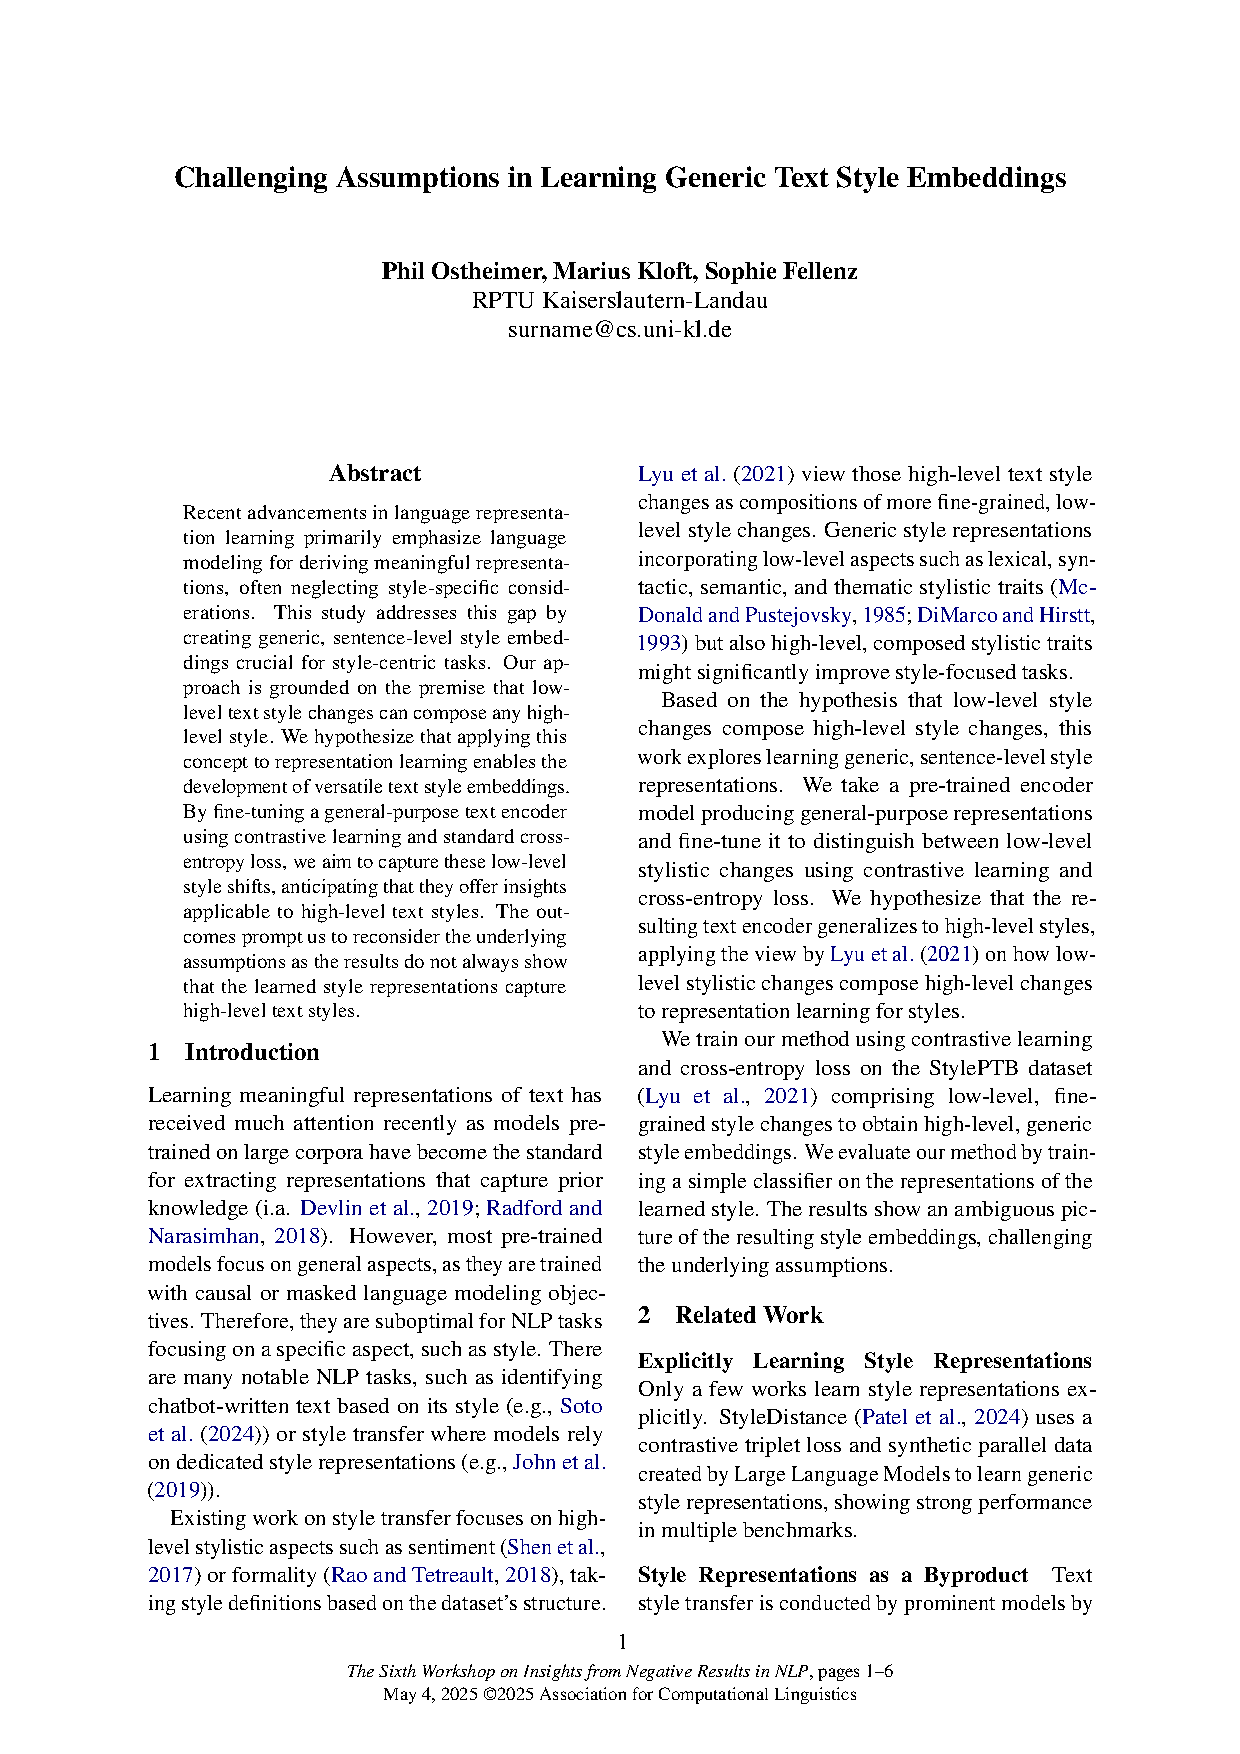
\includepdf[pagecommand={\thispagestyle{plain}},pages=-,addtotoc={1,section,1,{Challenging Assumptions in Learning Generic Text Style Embeddings},ref:paper_{1}}]{/home/blackbird/Projects_heavy/Research/Insight_Proceedings_2025/input/papers/1.pdf}
  \AddToShipoutPicture*{
    \setlength{\unitlength}{1mm}
    \footnotesize

            
    \put(0,13){\parbox[t]{\paperwidth}{\centering
    							\emph{The Sixth Workshop on Insights from Negative Results in NLP}, pages 7--14 \\
  	  						May 4, 2025 \textcopyright
  							2025 Association for Computational Linguistics}}
  }
  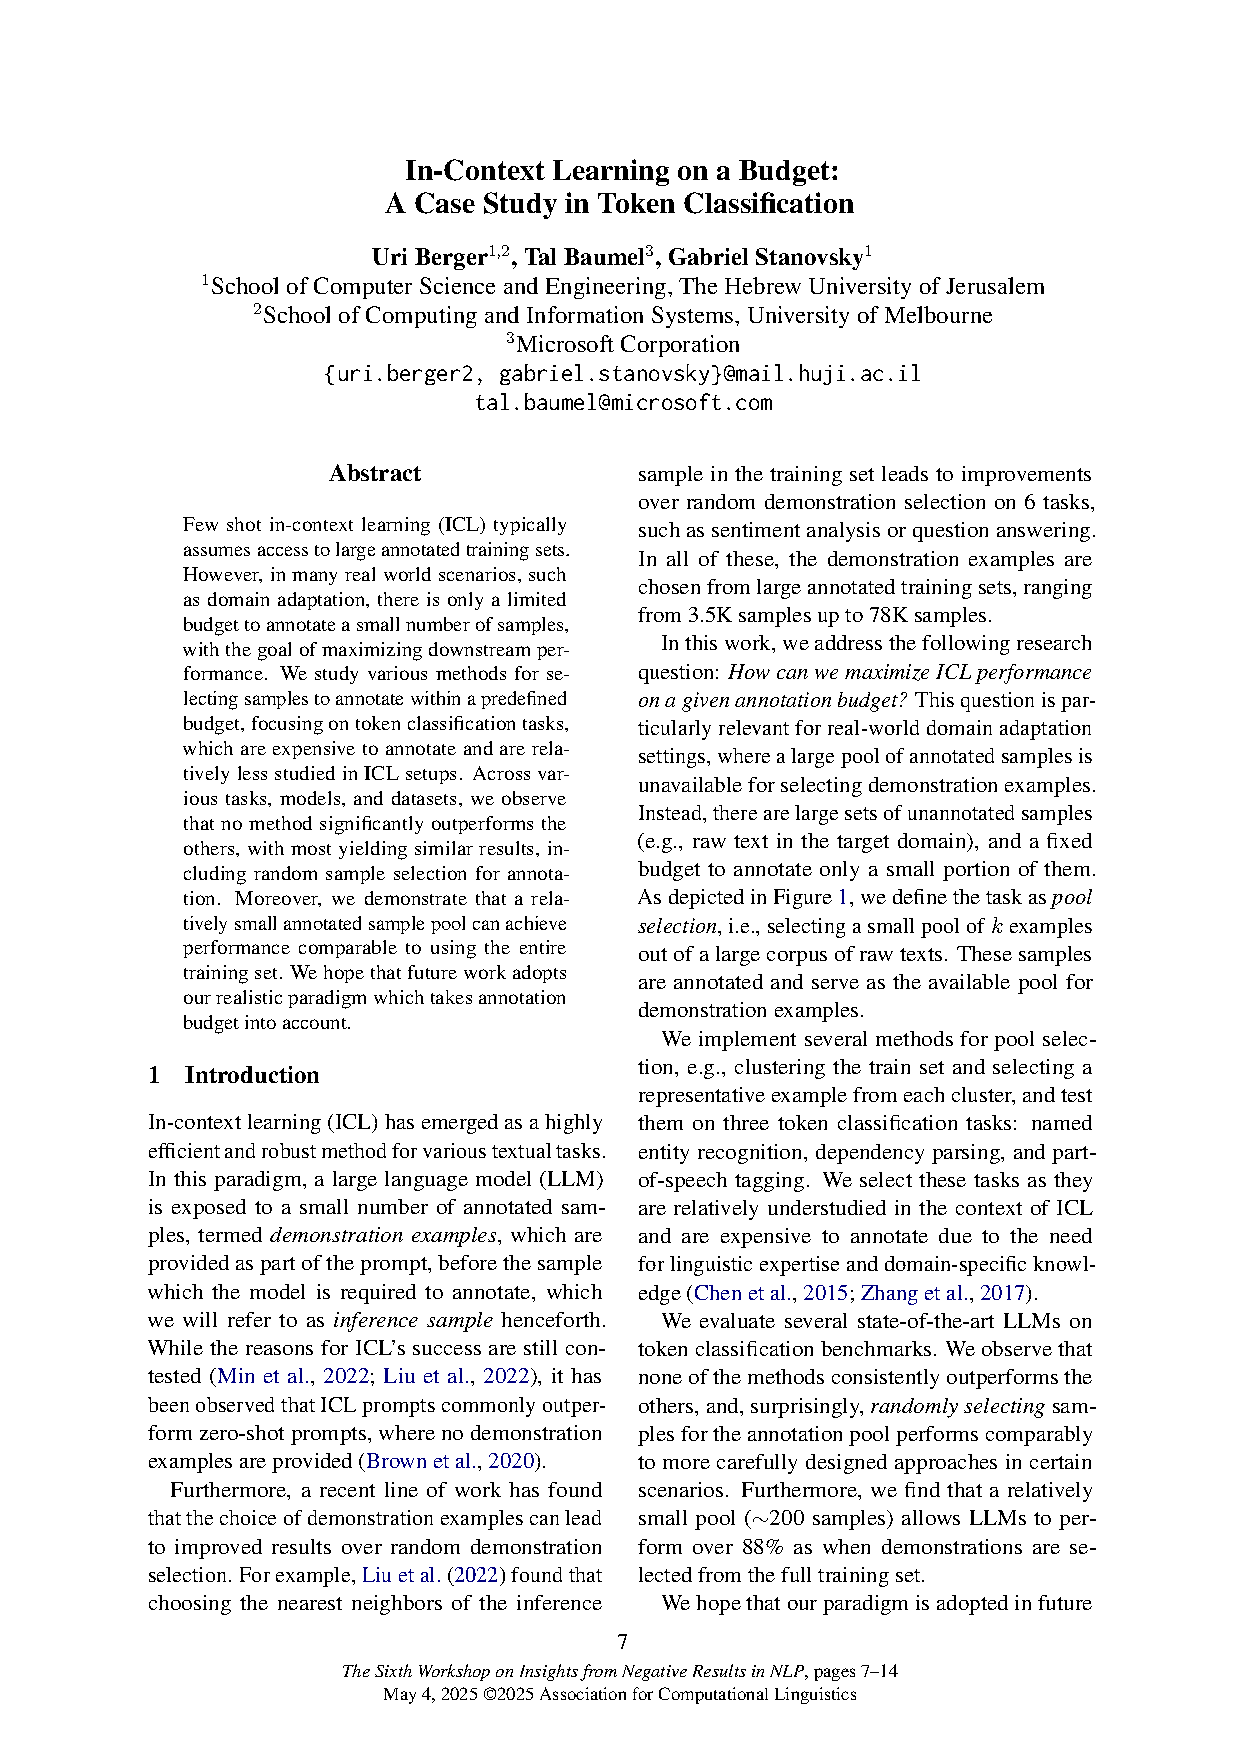
\includepdf[pagecommand={\thispagestyle{plain}},pages=-,addtotoc={1,section,1,{In-Context Learning on a Budget: A Case Study in Token Classification},ref:paper_{2}}]{/home/blackbird/Projects_heavy/Research/Insight_Proceedings_2025/input/papers/2.pdf}
  \AddToShipoutPicture*{
    \setlength{\unitlength}{1mm}
    \footnotesize

            
    \put(0,13){\parbox[t]{\paperwidth}{\centering
    							\emph{The Sixth Workshop on Insights from Negative Results in NLP}, pages 15--23 \\
  	  						May 4, 2025 \textcopyright
  							2025 Association for Computational Linguistics}}
  }
  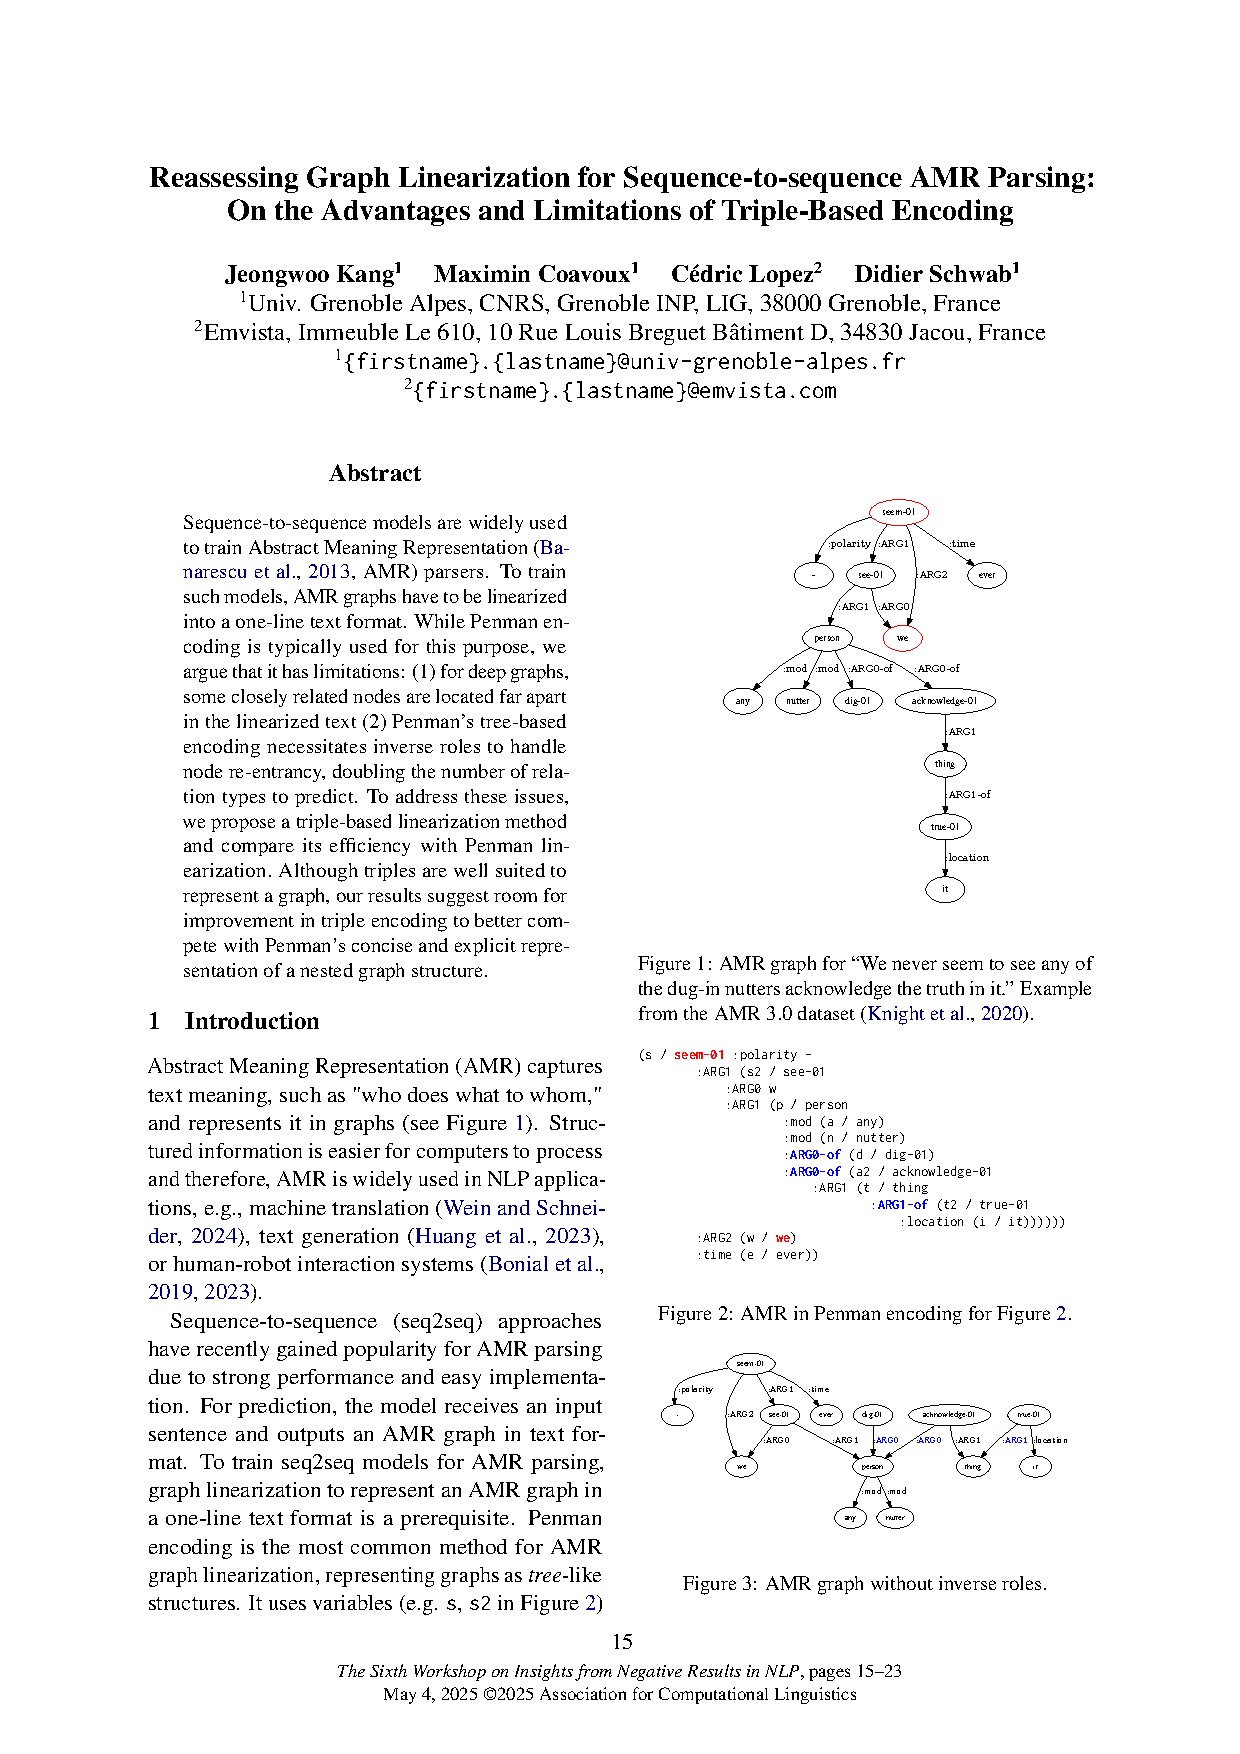
\includepdf[pagecommand={\thispagestyle{plain}},pages=-,addtotoc={1,section,1,{Reassessing Graph Linearization for Sequence-to-sequence AMR Parsing: On the Advantages and Limitations of Triple-Based},ref:paper_{4}}]{/home/blackbird/Projects_heavy/Research/Insight_Proceedings_2025/input/papers/4.pdf}
  \AddToShipoutPicture*{
    \setlength{\unitlength}{1mm}
    \footnotesize

            
    \put(0,13){\parbox[t]{\paperwidth}{\centering
    							\emph{The Sixth Workshop on Insights from Negative Results in NLP}, pages 24--33 \\
  	  						May 4, 2025 \textcopyright
  							2025 Association for Computational Linguistics}}
  }
  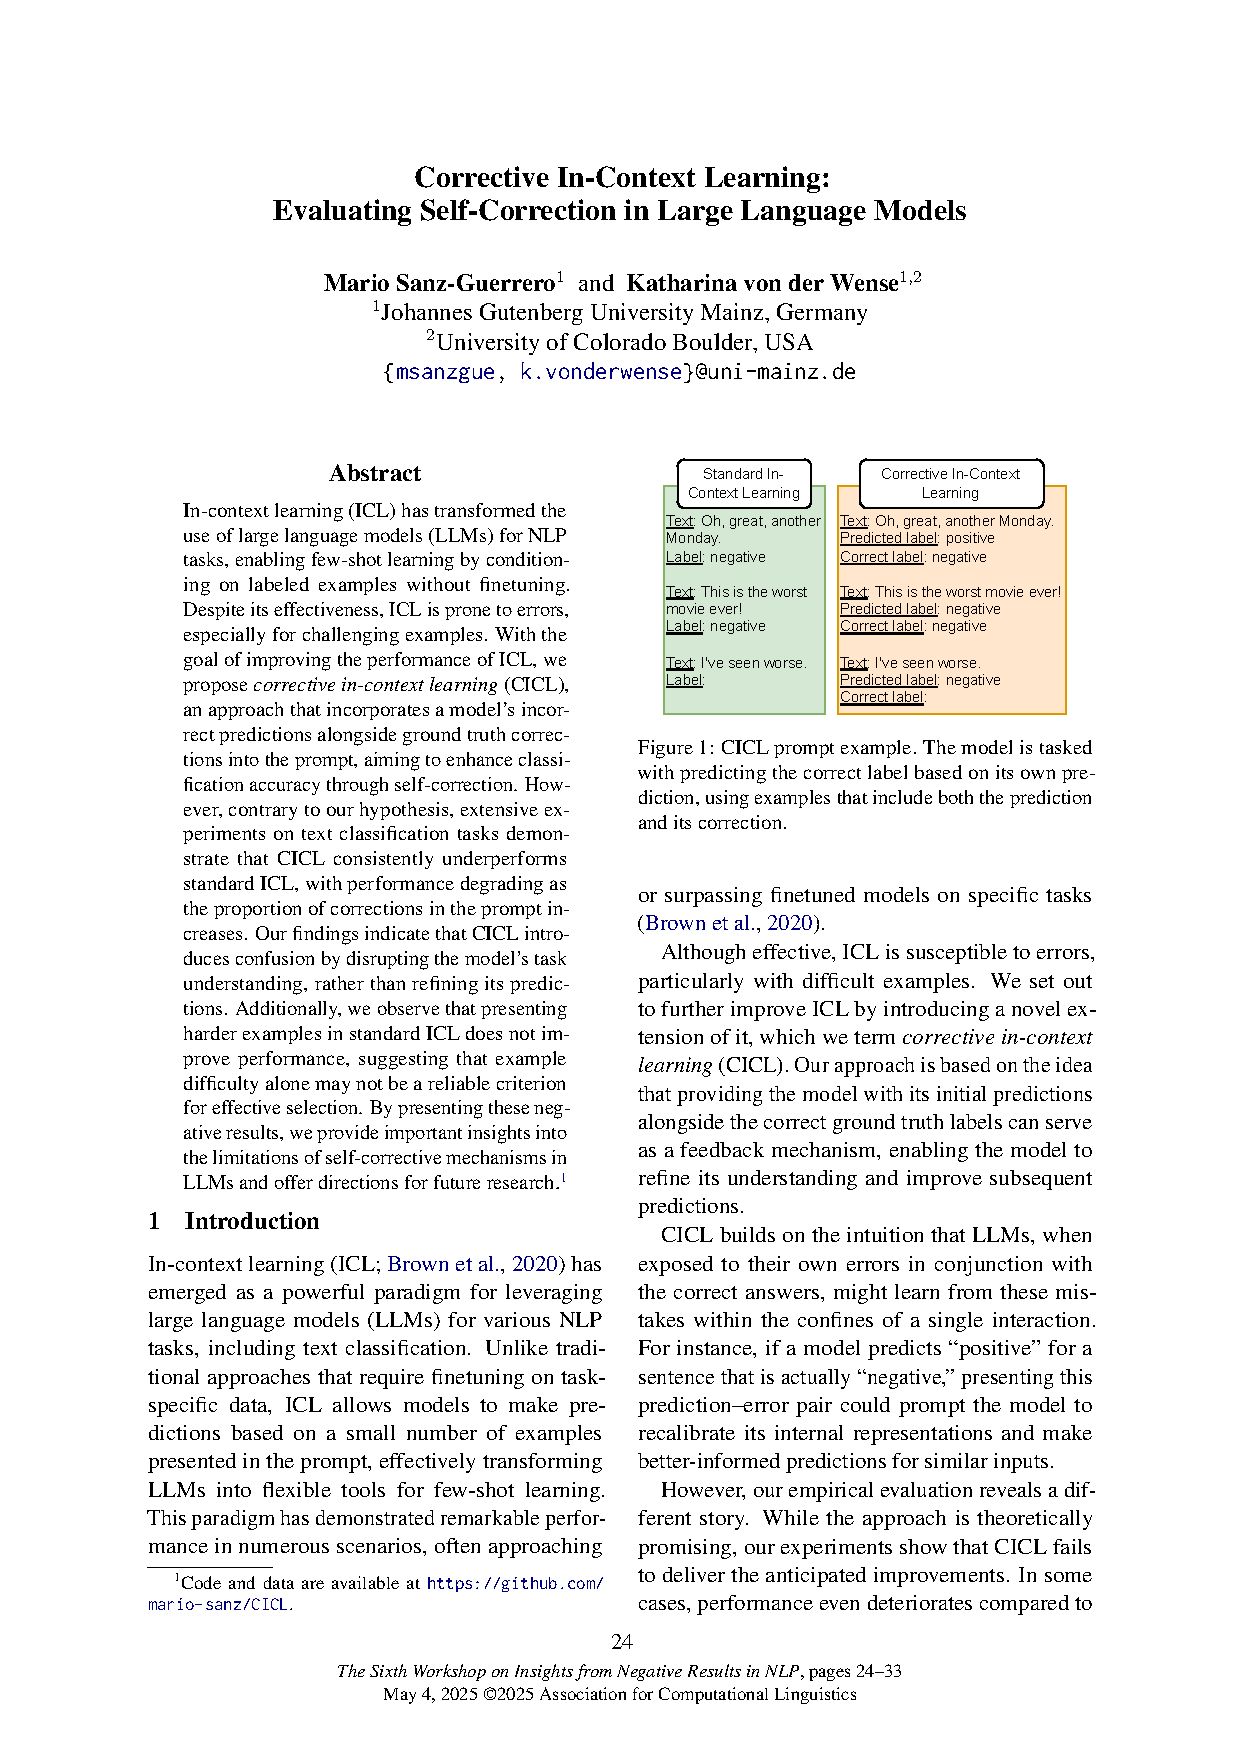
\includepdf[pagecommand={\thispagestyle{plain}},pages=-,addtotoc={1,section,1,{Corrective In-Context Learning: Evaluating Self-Correction in Large Language Models},ref:paper_{5}}]{/home/blackbird/Projects_heavy/Research/Insight_Proceedings_2025/input/papers/5.pdf}
  \AddToShipoutPicture*{
    \setlength{\unitlength}{1mm}
    \footnotesize

            
    \put(0,13){\parbox[t]{\paperwidth}{\centering
    							\emph{The Sixth Workshop on Insights from Negative Results in NLP}, pages 34--45 \\
  	  						May 4, 2025 \textcopyright
  							2025 Association for Computational Linguistics}}
  }
  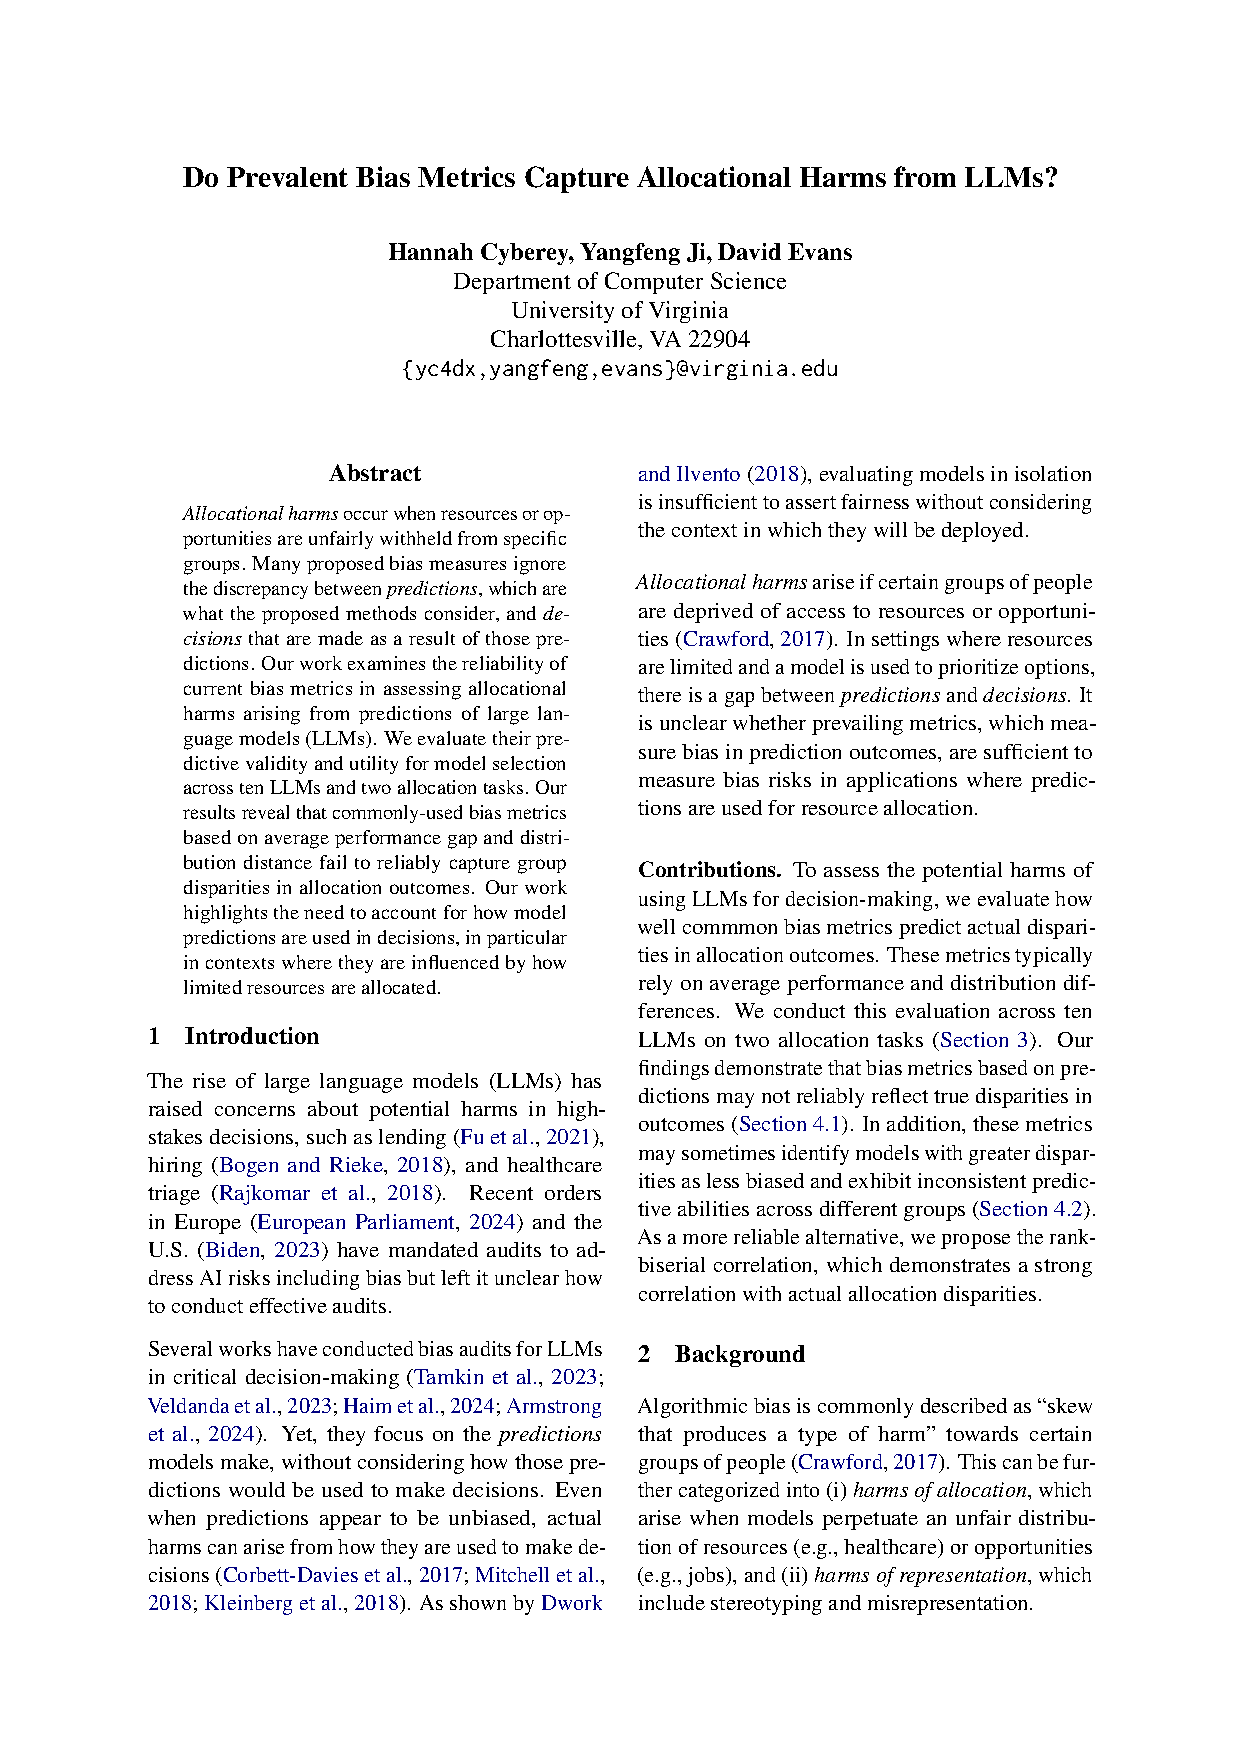
\includepdf[pagecommand={\thispagestyle{plain}},pages=-,addtotoc={1,section,1,{Do Prevalent Bias Metrics Capture Allocational Harms from LLMs?},ref:paper_{7}}]{/home/blackbird/Projects_heavy/Research/Insight_Proceedings_2025/input/papers/7.pdf}
  \AddToShipoutPicture*{
    \setlength{\unitlength}{1mm}
    \footnotesize

            
    \put(0,13){\parbox[t]{\paperwidth}{\centering
    							\emph{The Sixth Workshop on Insights from Negative Results in NLP}, pages 46--62 \\
  	  						May 4, 2025 \textcopyright
  							2025 Association for Computational Linguistics}}
  }
  \includepdf[pagecommand={\thispagestyle{plain}},pages=-,addtotoc={1,section,1,{Language-Specific Neurons Do Not Facilitate Cross-Lingual Transfer},ref:paper_{8}}]{/home/blackbird/Projects_heavy/Research/Insight_Proceedings_2025/input/papers/8.pdf}
  \AddToShipoutPicture*{
    \setlength{\unitlength}{1mm}
    \footnotesize

            
    \put(0,13){\parbox[t]{\paperwidth}{\centering
    							\emph{The Sixth Workshop on Insights from Negative Results in NLP}, pages 63--78 \\
  	  						May 4, 2025 \textcopyright
  							2025 Association for Computational Linguistics}}
  }
  \includepdf[pagecommand={\thispagestyle{plain}},pages=-,addtotoc={1,section,1,{Monte Carlo Sampling for Analyzing In-Context Examples},ref:paper_{10}}]{/home/blackbird/Projects_heavy/Research/Insight_Proceedings_2025/input/papers/10.pdf}
  \AddToShipoutPicture*{
    \setlength{\unitlength}{1mm}
    \footnotesize

            
    \put(0,13){\parbox[t]{\paperwidth}{\centering
    							\emph{The Sixth Workshop on Insights from Negative Results in NLP}, pages 79--85 \\
  	  						May 4, 2025 \textcopyright
  							2025 Association for Computational Linguistics}}
  }
  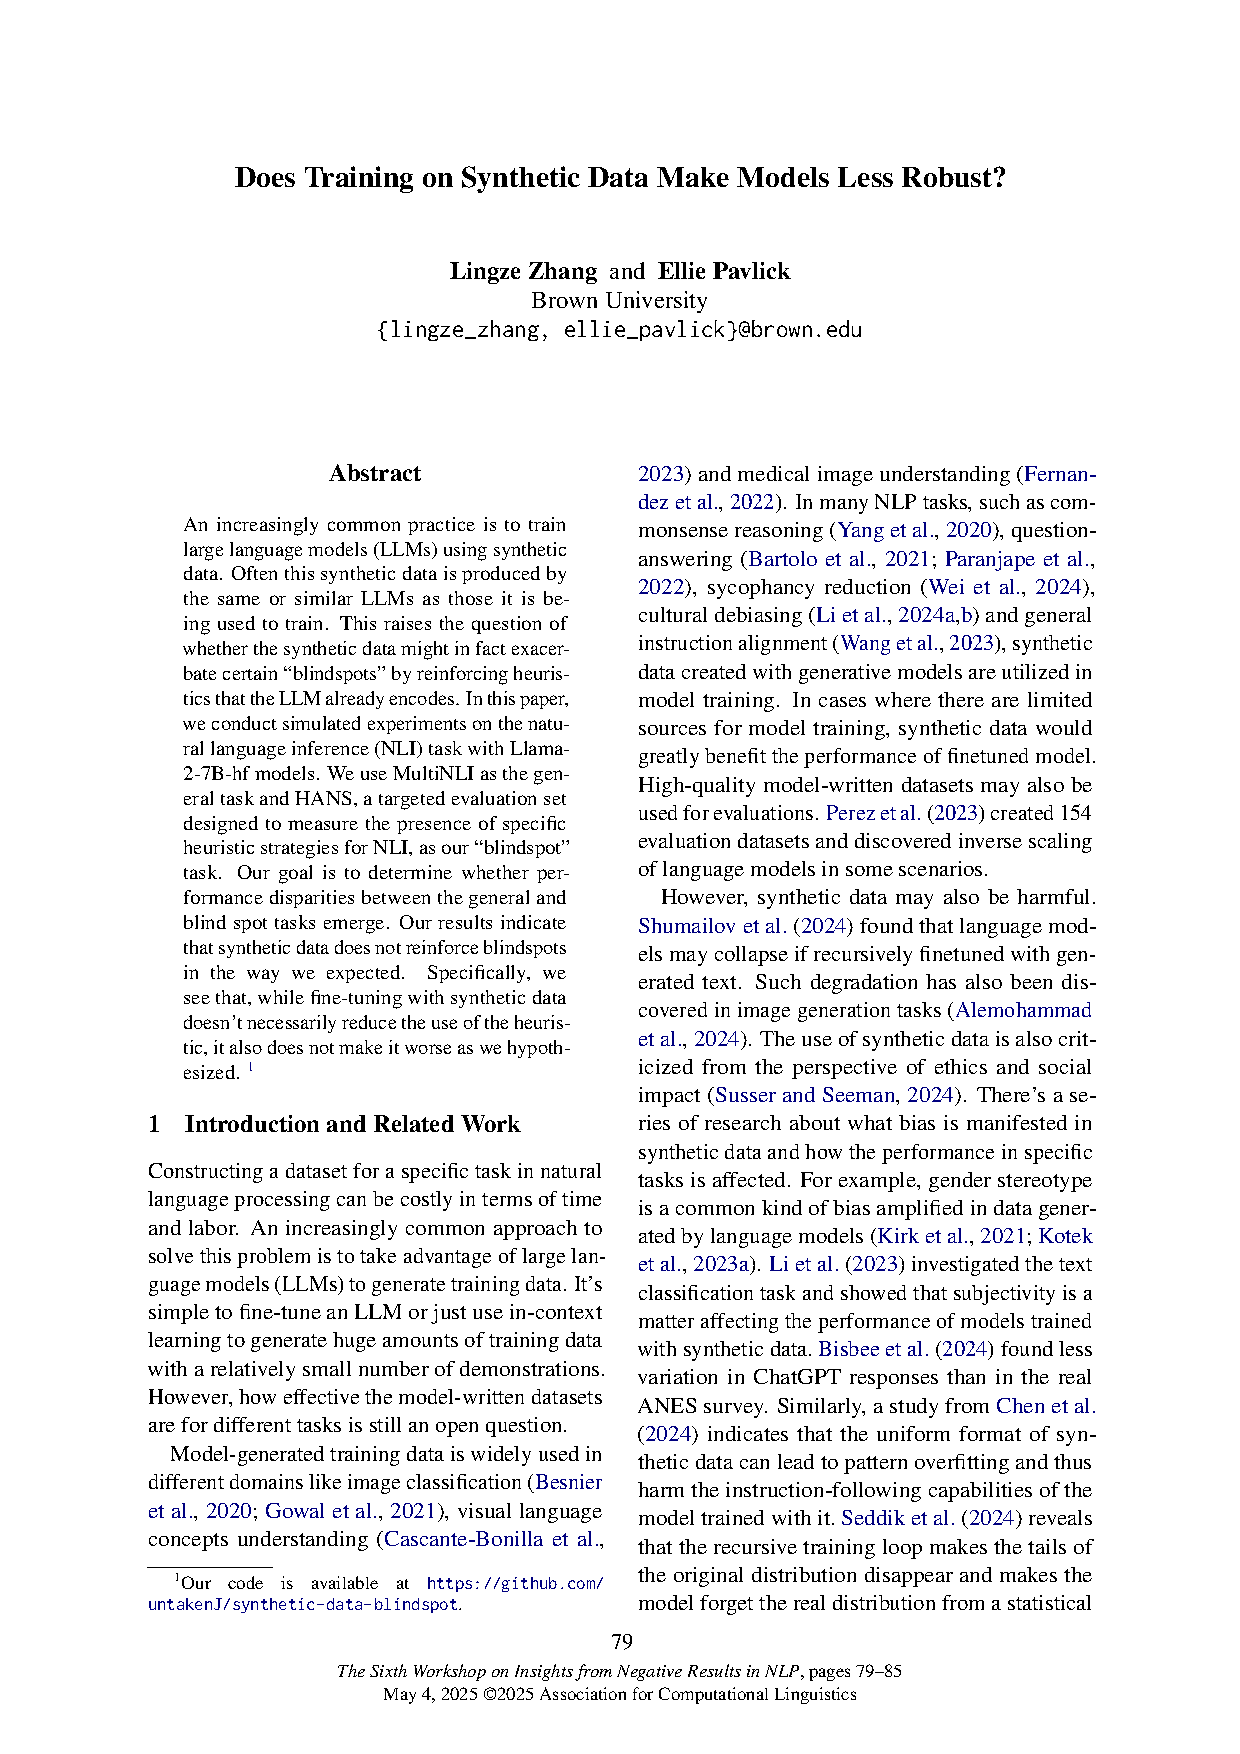
\includepdf[pagecommand={\thispagestyle{plain}},pages=-,addtotoc={1,section,1,{Does Training on Synthetic Data Make Models Less Robust?},ref:paper_{11}}]{/home/blackbird/Projects_heavy/Research/Insight_Proceedings_2025/input/papers/11.pdf}
  \AddToShipoutPicture*{
    \setlength{\unitlength}{1mm}
    \footnotesize

            
    \put(0,13){\parbox[t]{\paperwidth}{\centering
    							\emph{The Sixth Workshop on Insights from Negative Results in NLP}, pages 86--99 \\
  	  						May 4, 2025 \textcopyright
  							2025 Association for Computational Linguistics}}
  }
  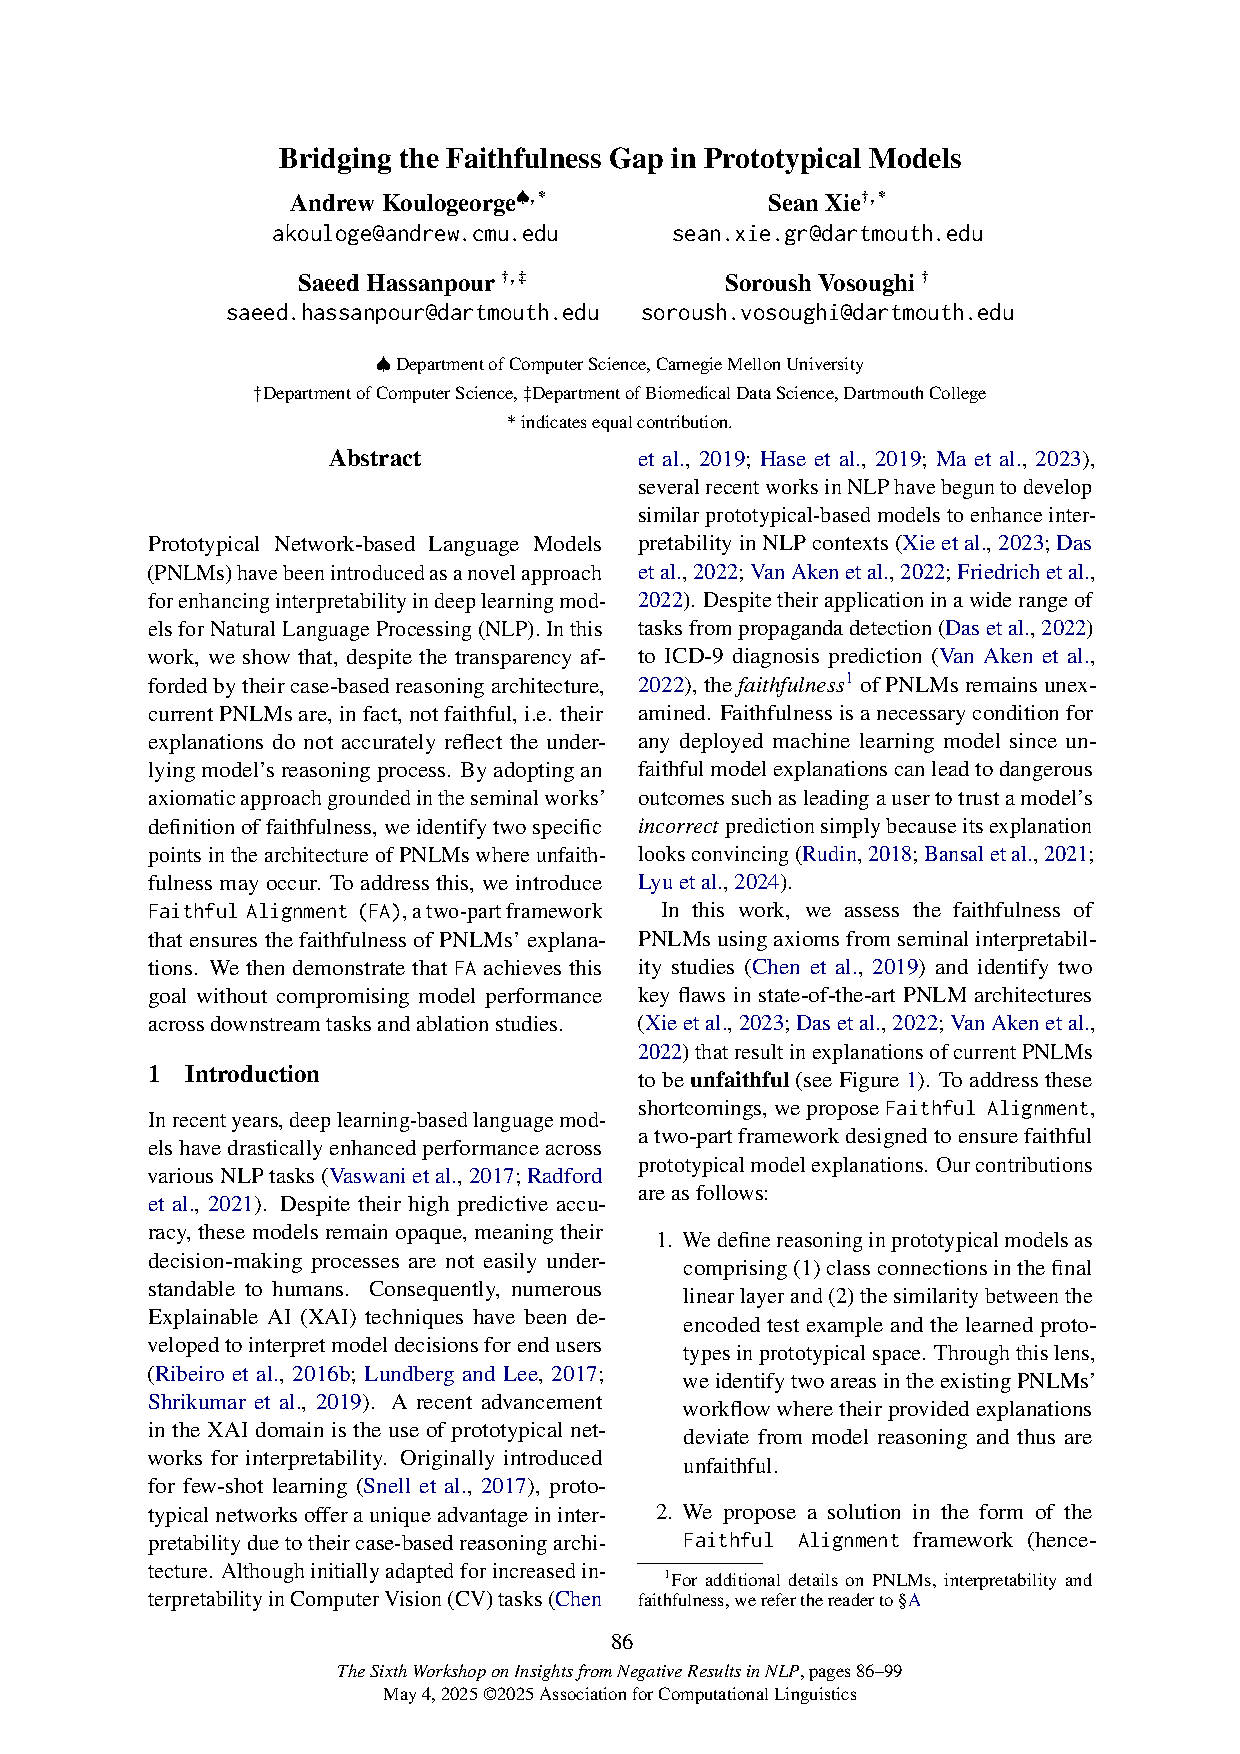
\includepdf[pagecommand={\thispagestyle{plain}},pages=-,addtotoc={1,section,1,{Bridging the Faithfulness Gap in Prototypical Models},ref:paper_{12}}]{/home/blackbird/Projects_heavy/Research/Insight_Proceedings_2025/input/papers/12.pdf}
  \AddToShipoutPicture*{
    \setlength{\unitlength}{1mm}
    \footnotesize

            
    \put(0,13){\parbox[t]{\paperwidth}{\centering
    							\emph{The Sixth Workshop on Insights from Negative Results in NLP}, pages 100--105 \\
  	  						May 4, 2025 \textcopyright
  							2025 Association for Computational Linguistics}}
  }
  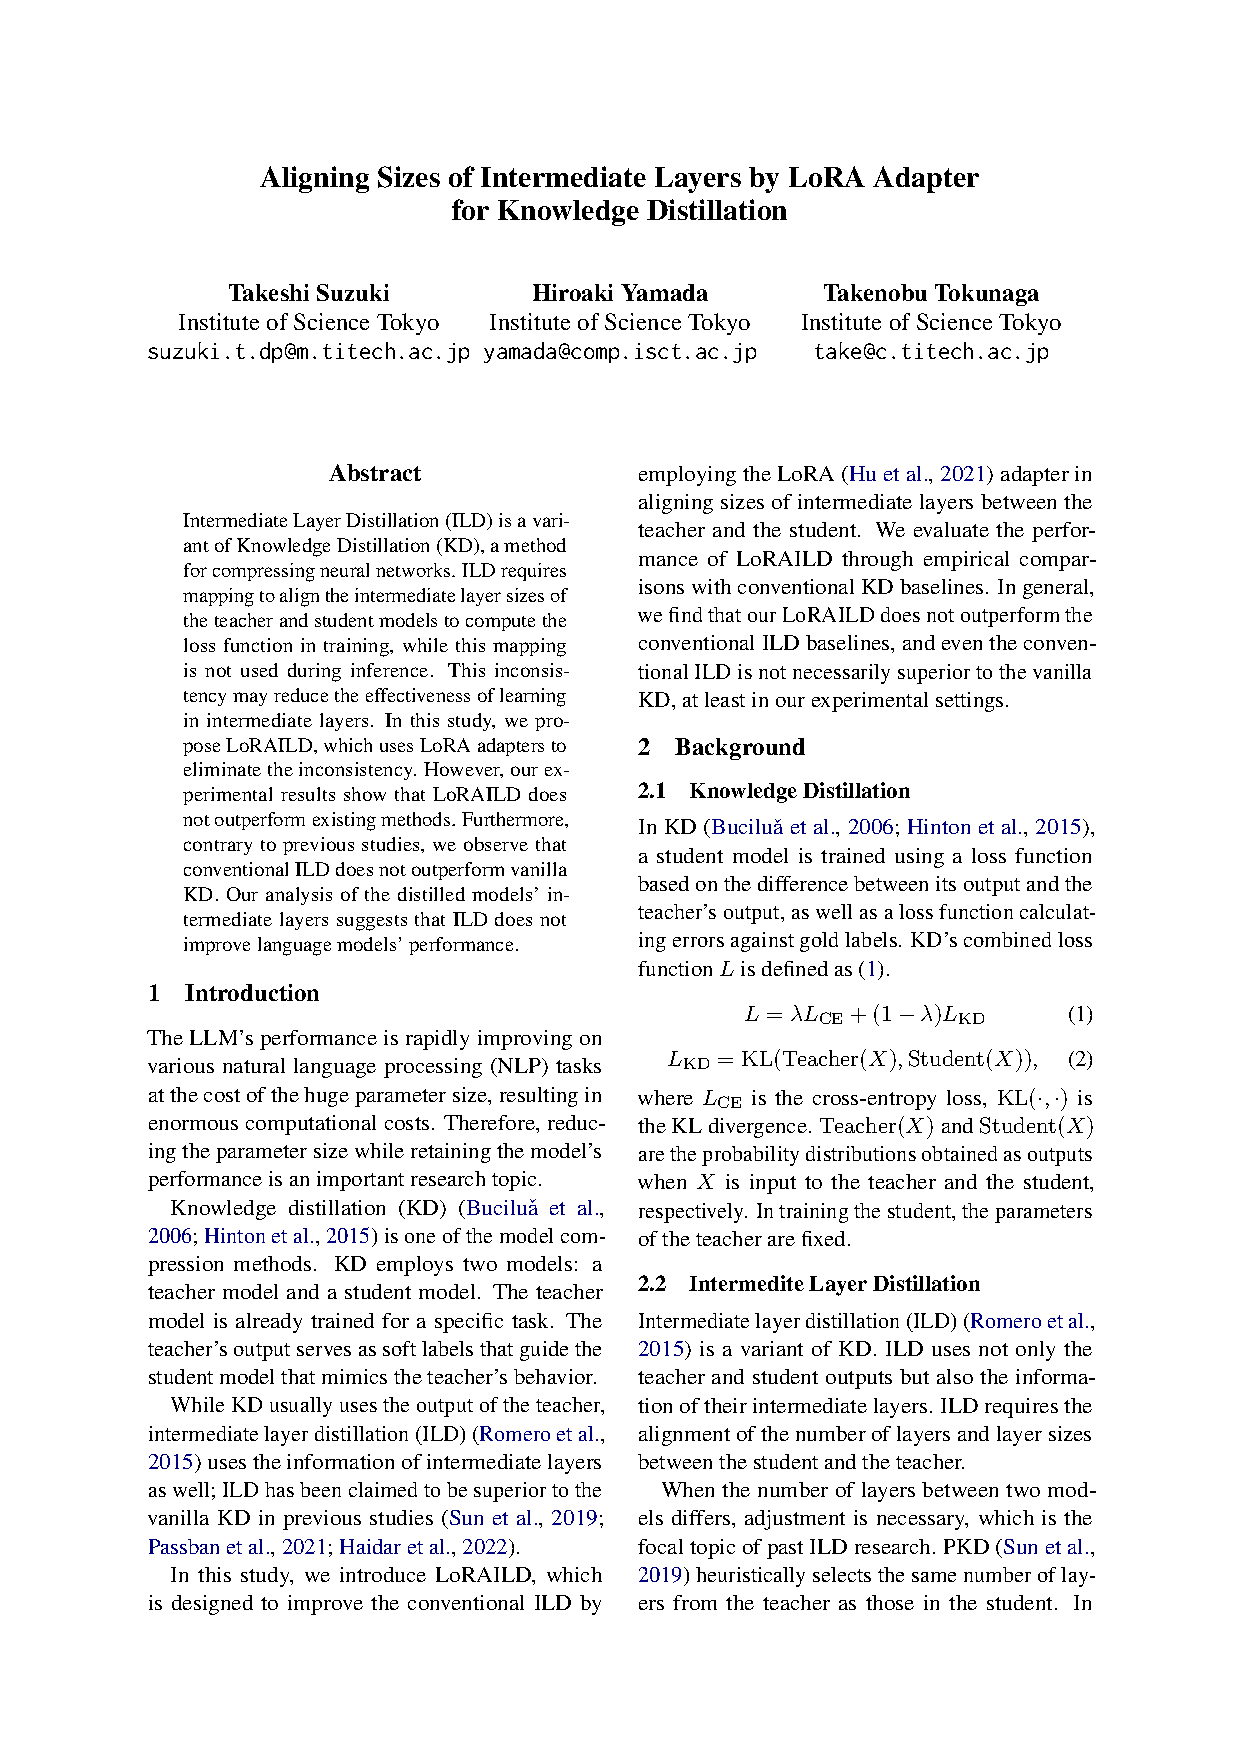
\includepdf[pagecommand={\thispagestyle{plain}},pages=-,addtotoc={1,section,1,{Aligning Sizes of Intermediate Layers by LoRA Adapter for Knowledge Distillation},ref:paper_{14}}]{/home/blackbird/Projects_heavy/Research/Insight_Proceedings_2025/input/papers/14.pdf}
  \AddToShipoutPicture*{
    \setlength{\unitlength}{1mm}
    \footnotesize

            
    \put(0,13){\parbox[t]{\paperwidth}{\centering
    							\emph{The Sixth Workshop on Insights from Negative Results in NLP}, pages 106--120 \\
  	  						May 4, 2025 \textcopyright
  							2025 Association for Computational Linguistics}}
  }
  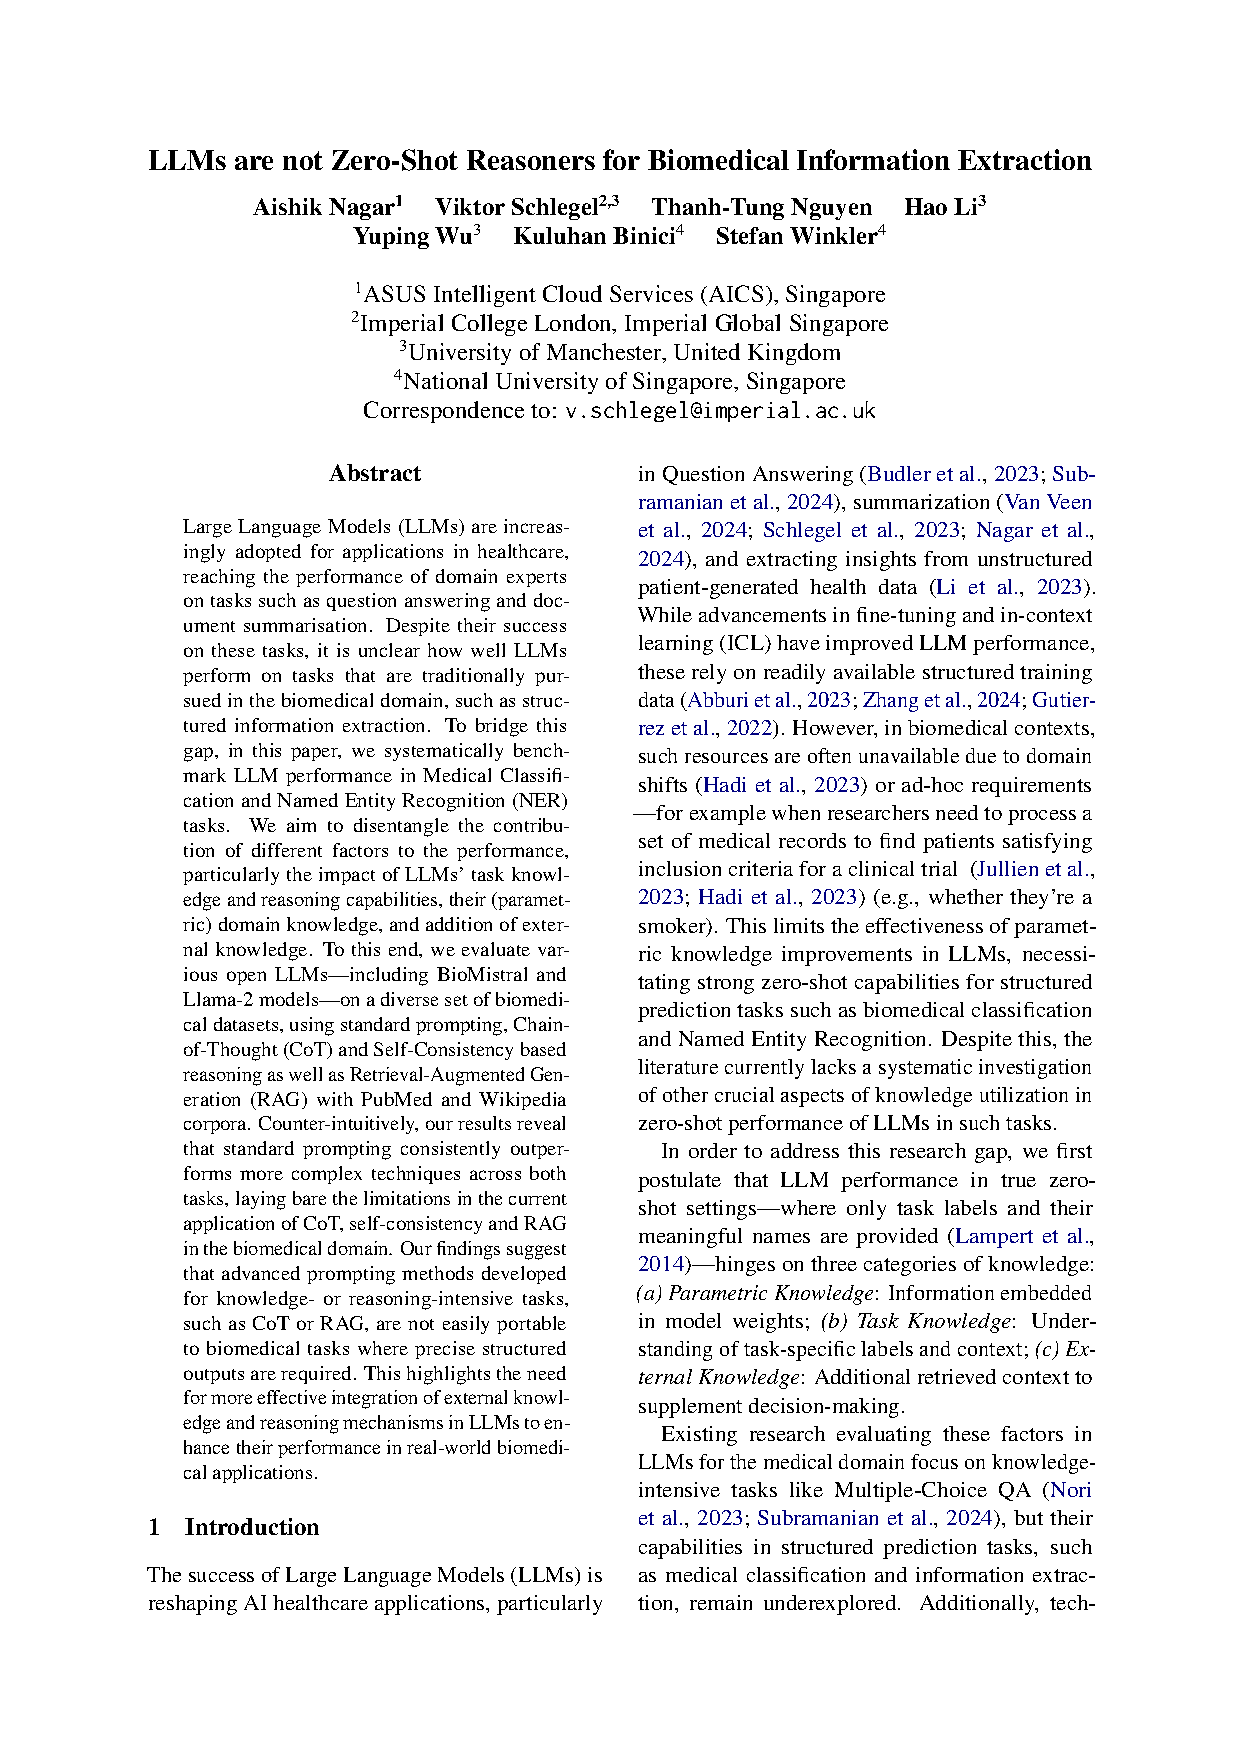
\includepdf[pagecommand={\thispagestyle{plain}},pages=-,addtotoc={1,section,1,{LLMs are not Zero-Shot Reasoners for Biomedical Information Extraction},ref:paper_{16}}]{/home/blackbird/Projects_heavy/Research/Insight_Proceedings_2025/input/papers/16.pdf}
  \AddToShipoutPicture*{
    \setlength{\unitlength}{1mm}
    \footnotesize

            
    \put(0,13){\parbox[t]{\paperwidth}{\centering
    							\emph{The Sixth Workshop on Insights from Negative Results in NLP}, pages 121--140 \\
  	  						May 4, 2025 \textcopyright
  							2025 Association for Computational Linguistics}}
  }
  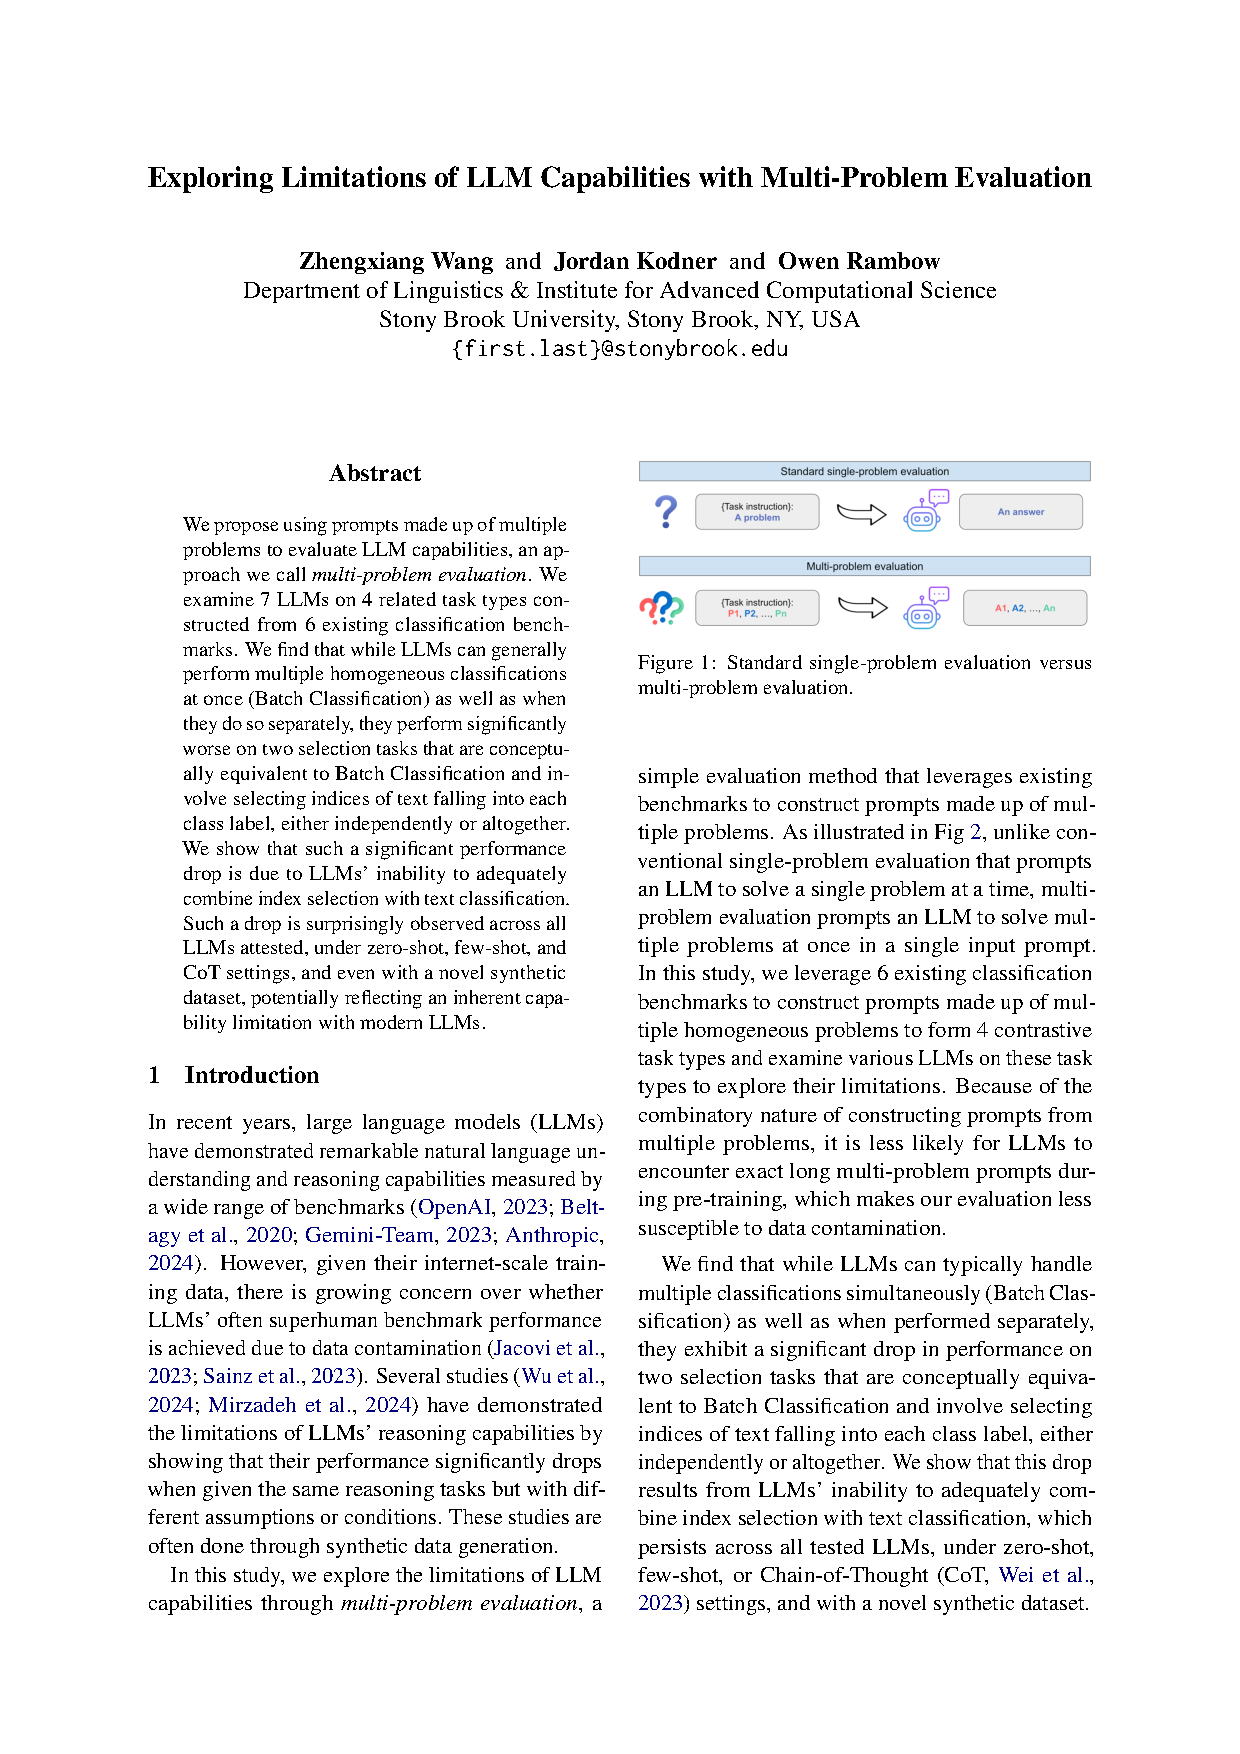
\includepdf[pagecommand={\thispagestyle{plain}},pages=-,addtotoc={1,section,1,{Exploring Limitations of LLM Capabilities with Multi-Problem Evaluation},ref:paper_{18}}]{/home/blackbird/Projects_heavy/Research/Insight_Proceedings_2025/input/papers/18.pdf}
  \AddToShipoutPicture*{
    \setlength{\unitlength}{1mm}
    \footnotesize

            
    \put(0,13){\parbox[t]{\paperwidth}{\centering
    							\emph{The Sixth Workshop on Insights from Negative Results in NLP}, pages 141--149 \\
  	  						May 4, 2025 \textcopyright
  							2025 Association for Computational Linguistics}}
  }
  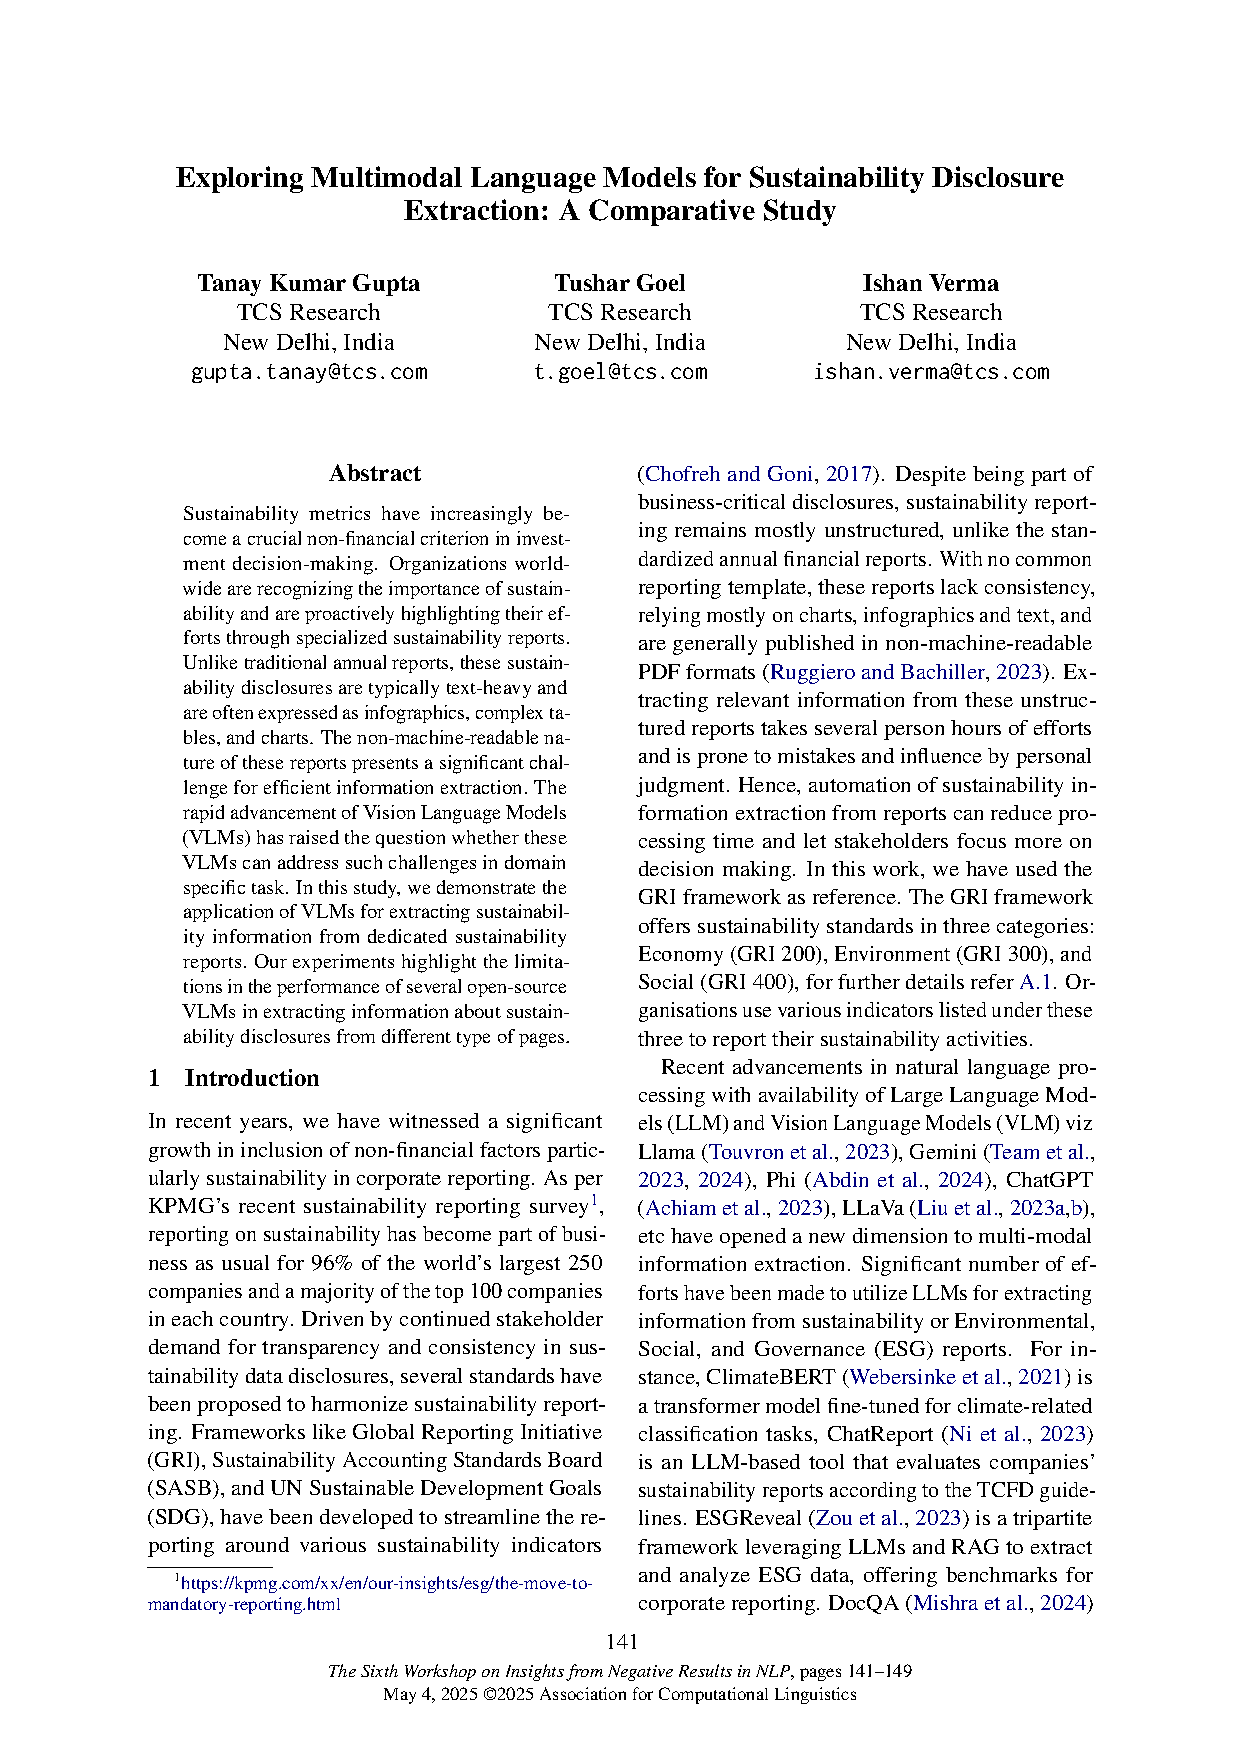
\includepdf[pagecommand={\thispagestyle{plain}},pages=-,addtotoc={1,section,1,{Exploring Multimodal Language Models for Sustainability Disclosure Extraction: A Comparative Study},ref:paper_{19}}]{/home/blackbird/Projects_heavy/Research/Insight_Proceedings_2025/input/papers/19.pdf}
  \AddToShipoutPicture*{
    \setlength{\unitlength}{1mm}
    \footnotesize

            
    \put(0,13){\parbox[t]{\paperwidth}{\centering
    							\emph{The Sixth Workshop on Insights from Negative Results in NLP}, pages 150--156 \\
  	  						May 4, 2025 \textcopyright
  							2025 Association for Computational Linguistics}}
  }
  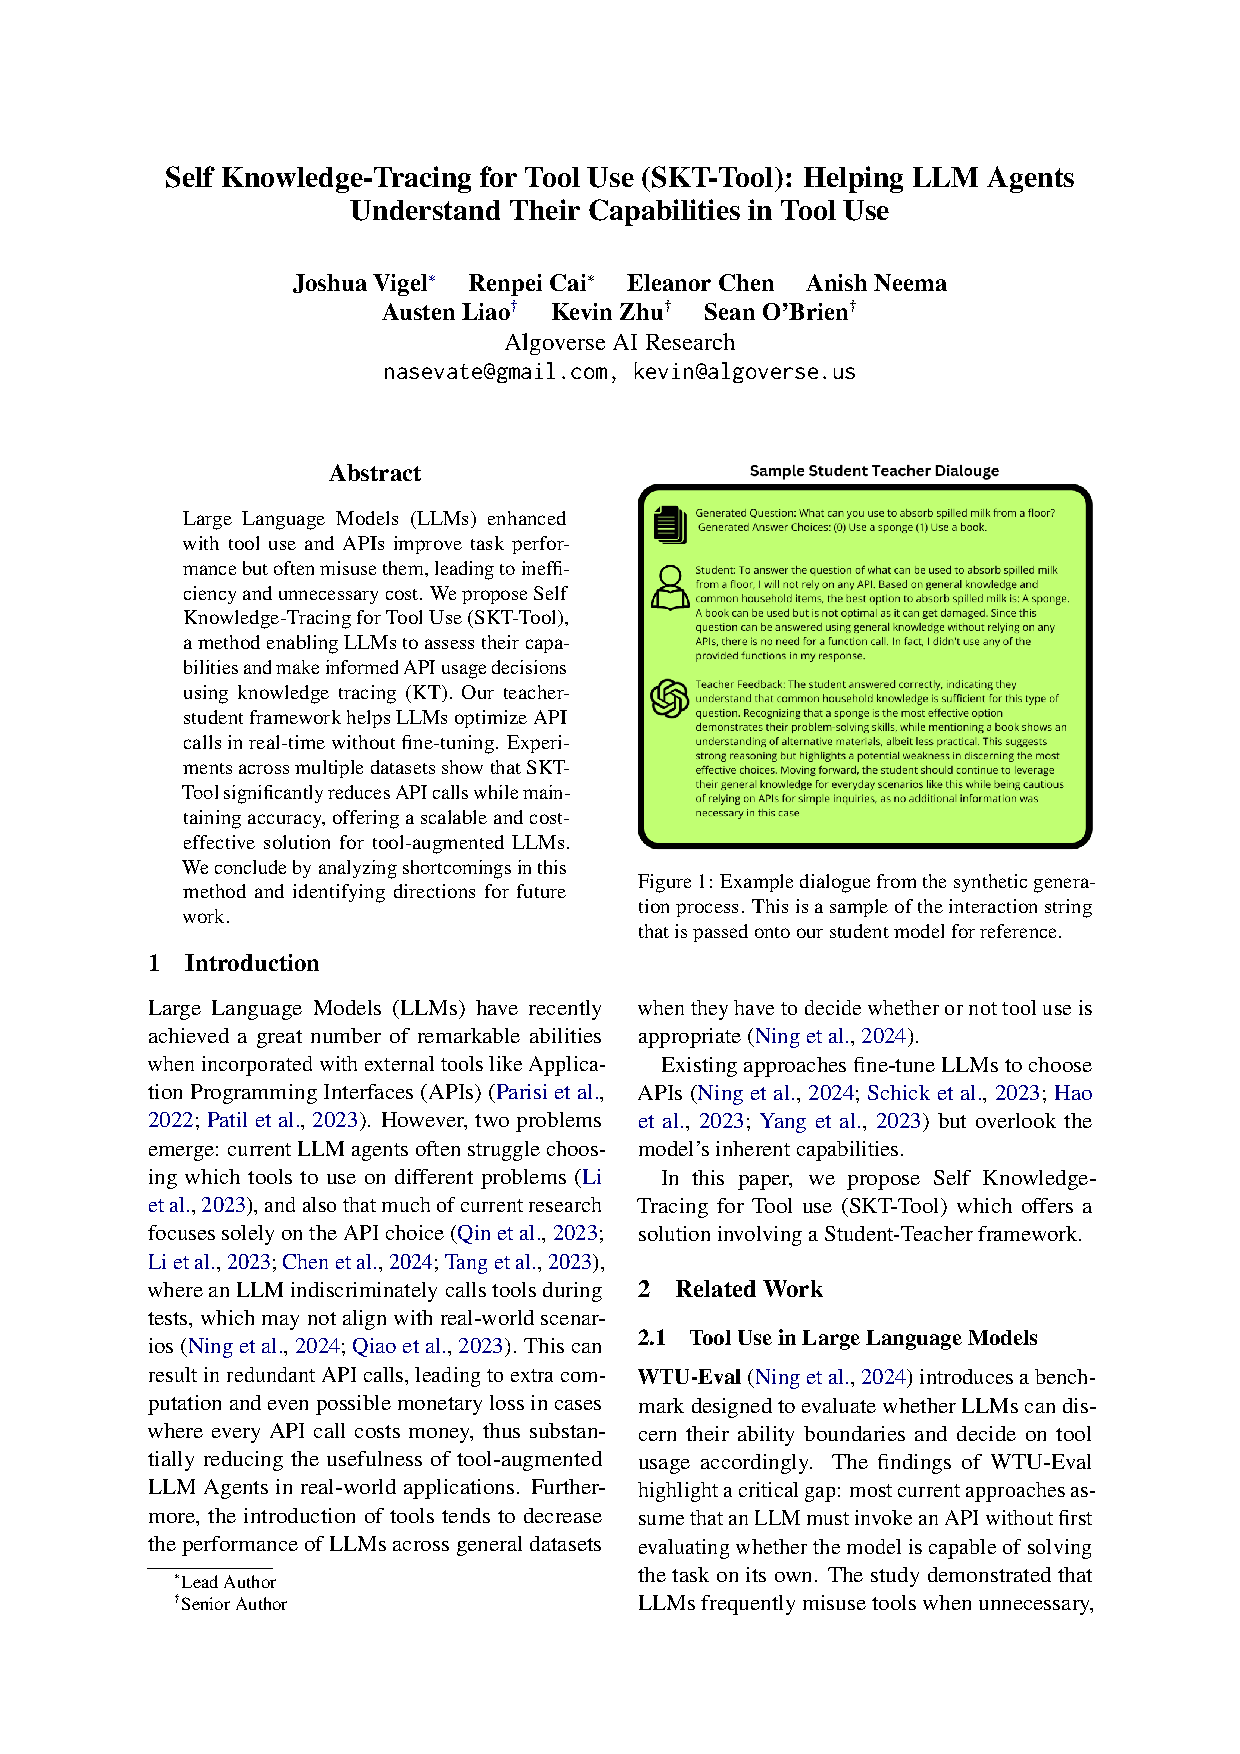
\includepdf[pagecommand={\thispagestyle{plain}},pages=-,addtotoc={1,section,1,{Self Knowledge-Tracing for Tool Use (SKT-Tool): Helping LLM Agents Understand Their Capabilities in Tool Use},ref:paper_{23}}]{/home/blackbird/Projects_heavy/Research/Insight_Proceedings_2025/input/papers/23.pdf}
  \AddToShipoutPicture*{
    \setlength{\unitlength}{1mm}
    \footnotesize

            
    \put(0,13){\parbox[t]{\paperwidth}{\centering
    							\emph{The Sixth Workshop on Insights from Negative Results in NLP}, pages 157--170 \\
  	  						May 4, 2025 \textcopyright
  							2025 Association for Computational Linguistics}}
  }
  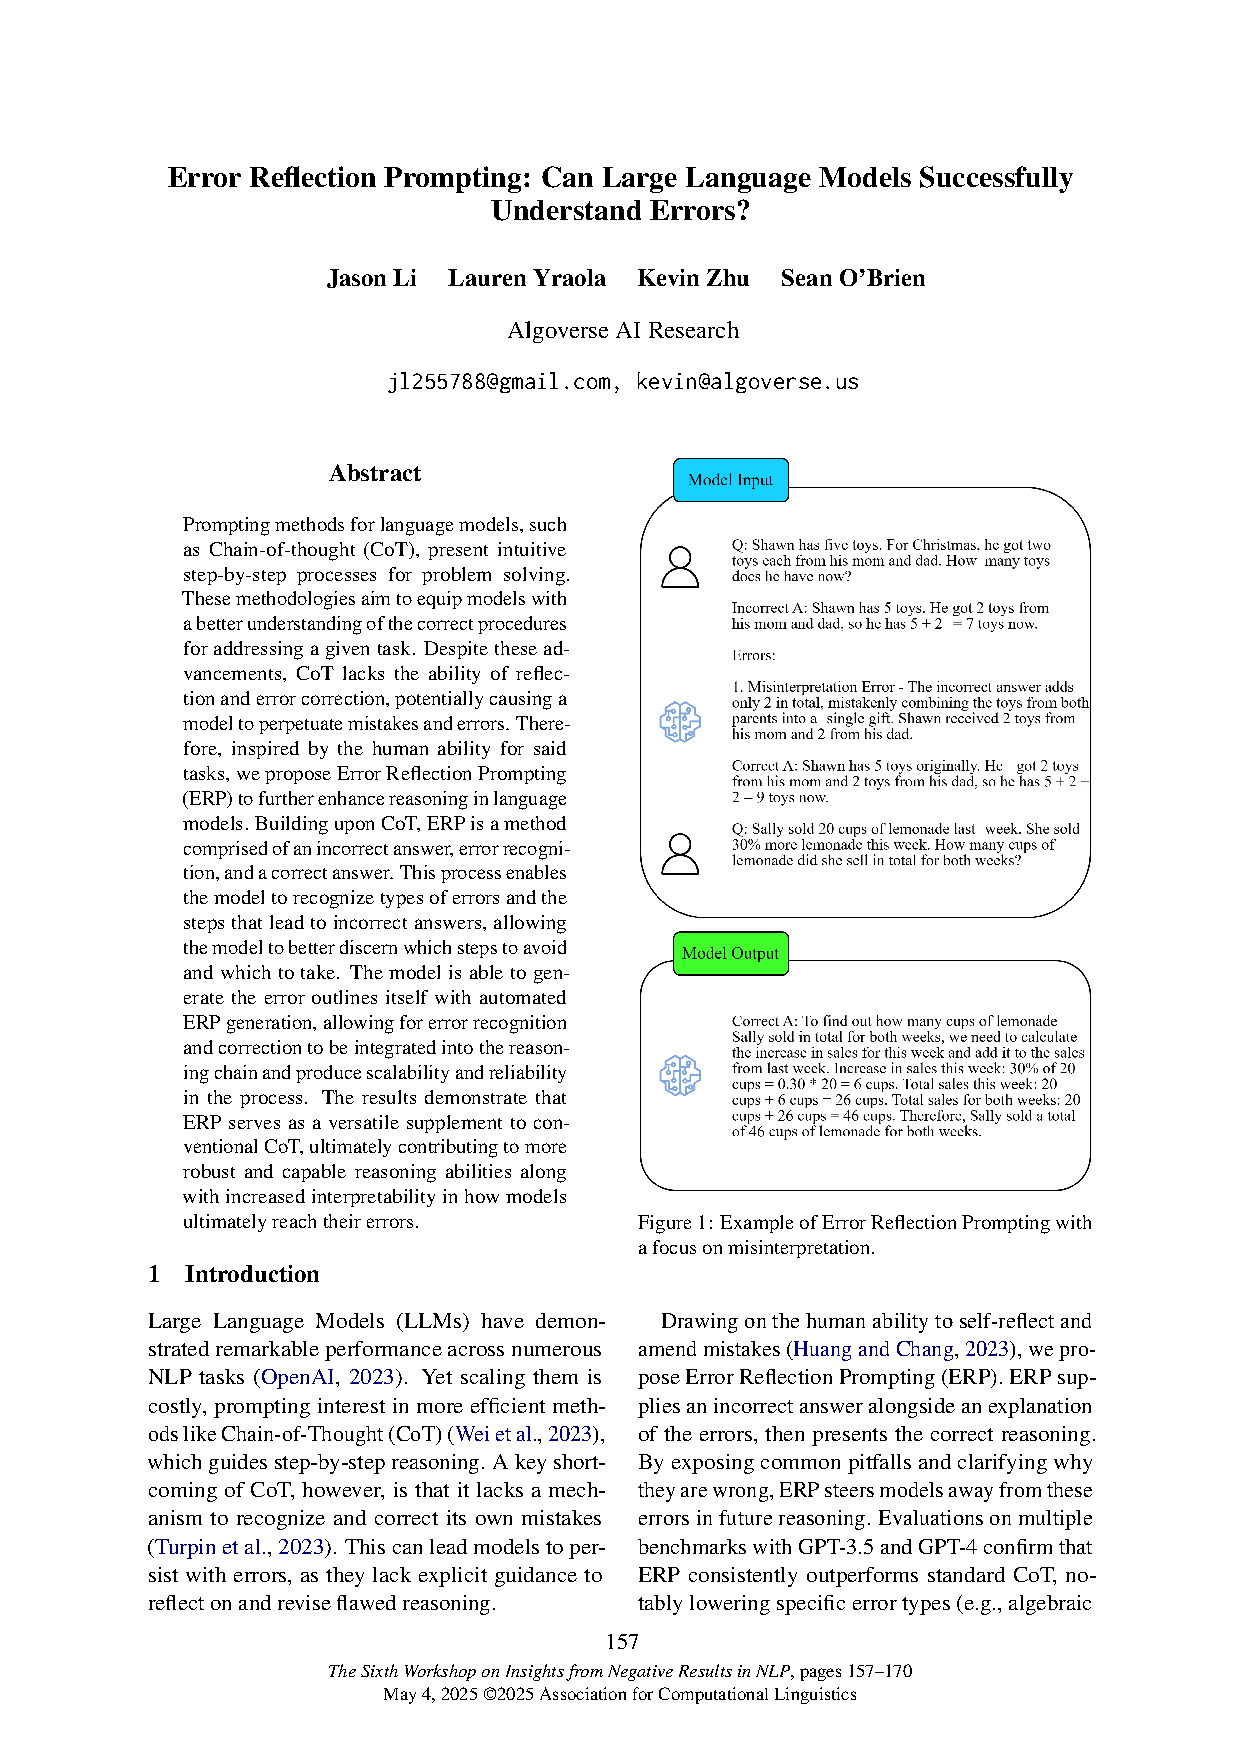
\includepdf[pagecommand={\thispagestyle{plain}},pages=-,addtotoc={1,section,1,{Error Reflection Prompting: Can Large Language Models Successfully Understand Errors?},ref:paper_{24}}]{/home/blackbird/Projects_heavy/Research/Insight_Proceedings_2025/input/papers/24.pdf}
  \AddToShipoutPicture*{
    \setlength{\unitlength}{1mm}
    \footnotesize

            
    \put(0,13){\parbox[t]{\paperwidth}{\centering
    							\emph{The Sixth Workshop on Insights from Negative Results in NLP}, pages 171--180 \\
  	  						May 4, 2025 \textcopyright
  							2025 Association for Computational Linguistics}}
  }
  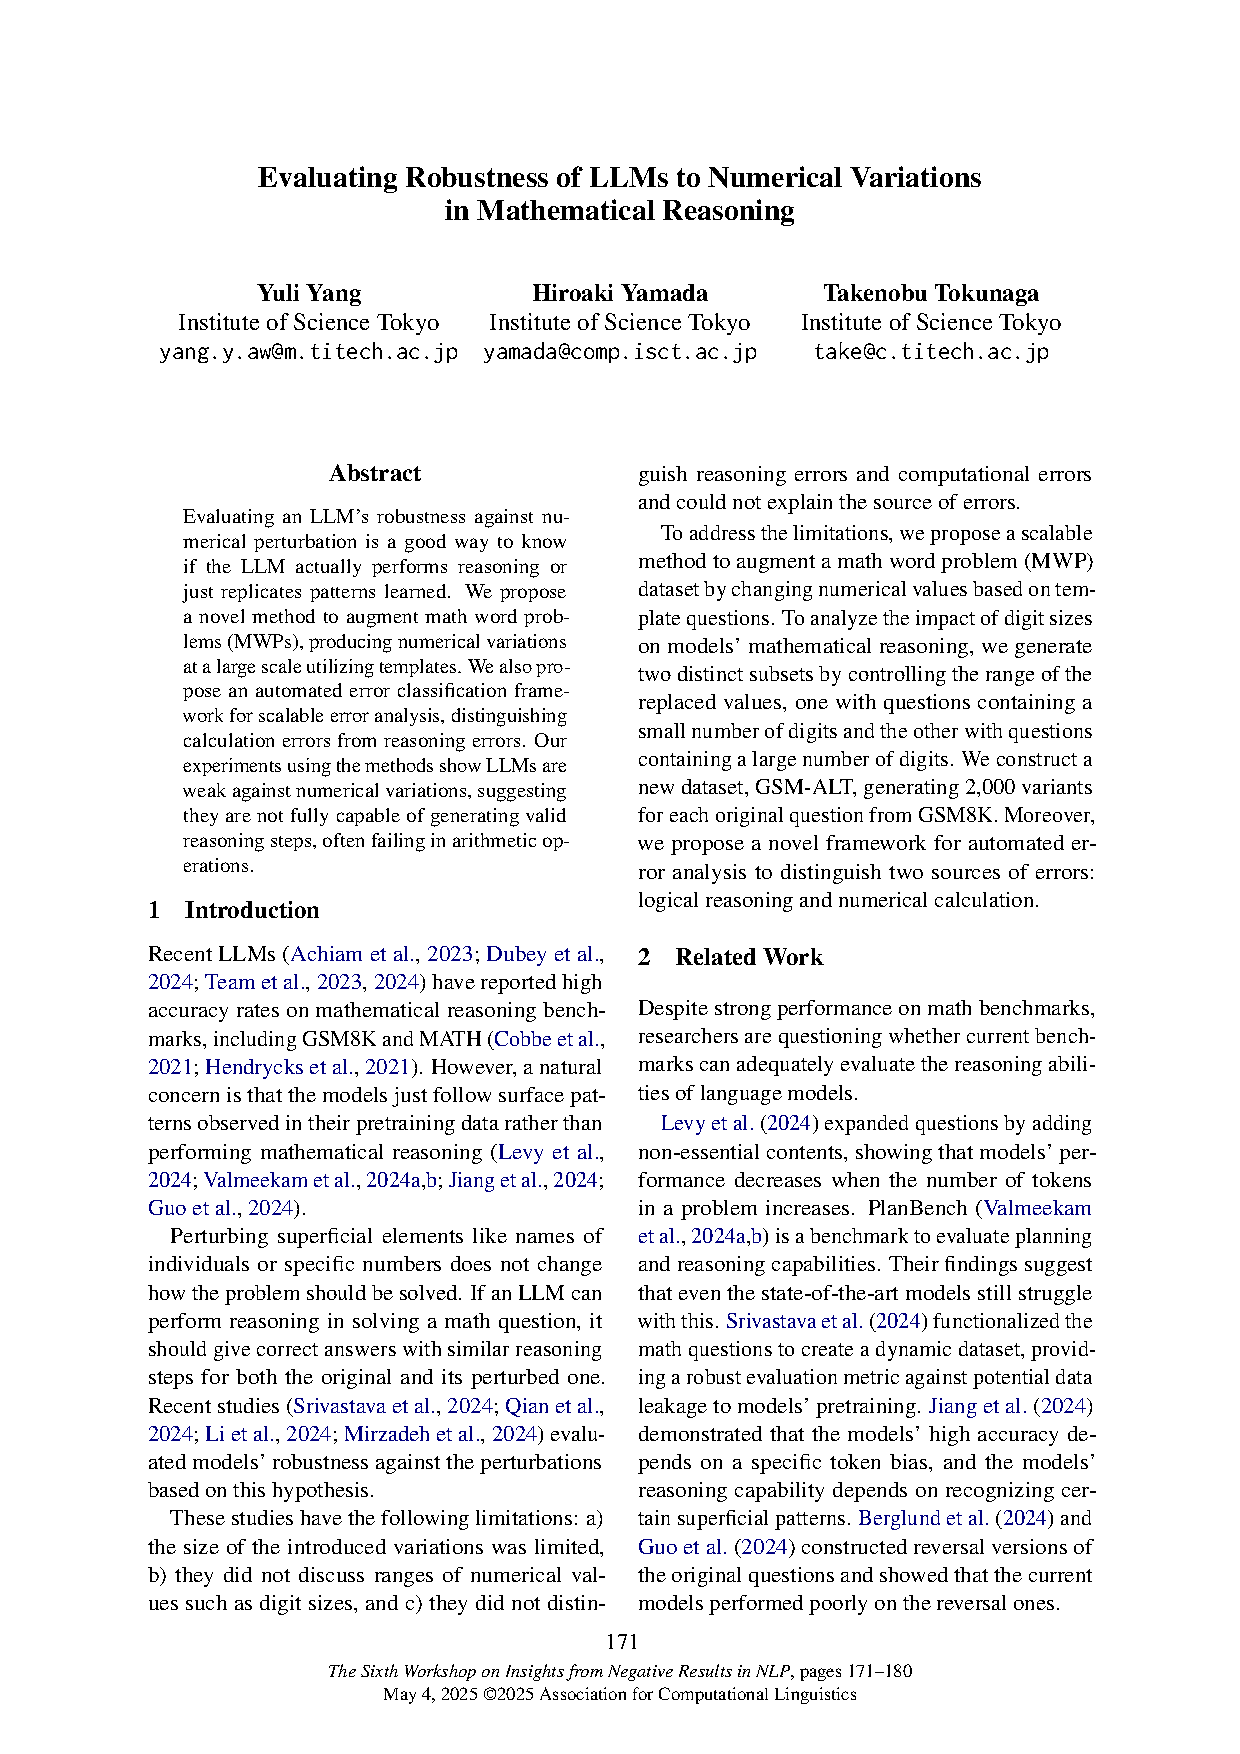
\includepdf[pagecommand={\thispagestyle{plain}},pages=-,addtotoc={1,section,1,{Evaluating Robustness of LLMs to Numerical Variations in Mathematical Reasoning},ref:paper_{25}}]{/home/blackbird/Projects_heavy/Research/Insight_Proceedings_2025/input/papers/25.pdf}

%%%%%%%%%%%%%%%%
% Author Index %
%%%%%%%%%%%%%%%%
\begin{huge}
Author Index
\end{huge}
\vspace*{1em}
\begin{multicols}{2}
Baumel, Tal, \hyperlink{page.7}{7}\\
Berger, Uri, \hyperlink{page.7}{7}\\
Binici, Kuluhan, \hyperlink{page.106}{106}\\
\\ % Extra space between new letters.
Cai, Renpei, \hyperlink{page.150}{150}\\
Chen, Eleanor, \hyperlink{page.150}{150}\\
Coavoux, Maximin, \hyperlink{page.15}{15}\\
Cyberey, Hannah, \hyperlink{page.34}{34}\\
\\ % Extra space between new letters.
Evans, David, \hyperlink{page.34}{34}\\
\\ % Extra space between new letters.
Fellenz, Sophie, \hyperlink{page.1}{1}\\
\\ % Extra space between new letters.
Goel, Tushar, \hyperlink{page.141}{141}\\
Gupta, Tanay, \hyperlink{page.141}{141}\\
\\ % Extra space between new letters.
Hassanpour, Saeed, \hyperlink{page.86}{86}\\
\\ % Extra space between new letters.
Ji, Yangfeng, \hyperlink{page.34}{34}, \hyperlink{page.63}{63}\\
Jyothi, Preethi, \hyperlink{page.46}{46}\\
\\ % Extra space between new letters.
Kang, Jeongwoo, \hyperlink{page.15}{15}\\
Kloft, Marius, \hyperlink{page.1}{1}\\
Kodner, Jordan, \hyperlink{page.121}{121}\\
Koulogeorge, Andrew, \hyperlink{page.86}{86}\\
\\ % Extra space between new letters.
Li, Hao, \hyperlink{page.106}{106}\\
Li, Jason, \hyperlink{page.157}{157}\\
Liao, Austen, \hyperlink{page.150}{150}\\
Lopez, Cédric, \hyperlink{page.15}{15}\\
\\ % Extra space between new letters.
Mondal, Soumen Kumar, \hyperlink{page.46}{46}\\
\\ % Extra space between new letters.
Nagar, Aishik, \hyperlink{page.106}{106}\\
Neema, Anish, \hyperlink{page.150}{150}\\
Nguyen, T h a n h - T u n g, \hyperlink{page.106}{106}\\
\\ % Extra space between new letters.
O'brien, Sean, \hyperlink{page.150}{150}, \hyperlink{page.157}{157}\\
Ostheimer, Phil, \hyperlink{page.1}{1}\\
\\ % Extra space between new letters.
Pavlick, Ellie, \hyperlink{page.79}{79}\\
\\ % Extra space between new letters.
Rambow, Owen, \hyperlink{page.121}{121}\\
\\ % Extra space between new letters.
S a n z - G u e r r e r o, Mario, \hyperlink{page.24}{24}\\
Schlegel, Viktor, \hyperlink{page.106}{106}\\
Schoch, Stephanie, \hyperlink{page.63}{63}\\
Schwab, Didier, \hyperlink{page.15}{15}\\
Sen, Sayambhu, \hyperlink{page.46}{46}\\
Singhania, Abhishek, \hyperlink{page.46}{46}\\
Stanovsky, Gabriel, \hyperlink{page.7}{7}\\
Suzuki, Takeshi, \hyperlink{page.100}{100}\\
\\ % Extra space between new letters.
Tokunaga, Takenobu, \hyperlink{page.100}{100}, \hyperlink{page.171}{171}\\
\\ % Extra space between new letters.
Verma, Ishan, \hyperlink{page.141}{141}\\
Vigel, Joshua, \hyperlink{page.150}{150}\\
Von Der Wense, Katharina, \hyperlink{page.24}{24}\\
Vosoughi, Soroush, \hyperlink{page.86}{86}\\
\\ % Extra space between new letters.
Wang, Zhengxiang, \hyperlink{page.121}{121}\\
Winkler, Stefan, \hyperlink{page.106}{106}\\
Wu, Yuping, \hyperlink{page.106}{106}\\
\\ % Extra space between new letters.
Xie, Sean, \hyperlink{page.86}{86}\\
\\ % Extra space between new letters.
Yamada, Hiroaki, \hyperlink{page.100}{100}, \hyperlink{page.171}{171}\\
Yang, Yuli, \hyperlink{page.171}{171}\\
Yraola, Lauren, \hyperlink{page.157}{157}\\
\\ % Extra space between new letters.
Zhang, Lingze, \hyperlink{page.79}{79}\\
Zhu, Kevin, \hyperlink{page.150}{150}, \hyperlink{page.157}{157}\\
\\ % Extra space between new letters.
\end{multicols}


\end{document}